\documentclass[1p]{elsarticle_modified}
%\bibliographystyle{elsarticle-num}

%\usepackage[colorlinks]{hyperref}
%\usepackage{abbrmath_seonhwa} %\Abb, \Ascr, \Acal ,\Abf, \Afrak
\usepackage{amsfonts}
\usepackage{amssymb}
\usepackage{amsmath}
\usepackage{amsthm}
\usepackage{scalefnt}
\usepackage{amsbsy}
\usepackage{kotex}
\usepackage{caption}
\usepackage{subfig}
\usepackage{color}
\usepackage{graphicx}
\usepackage{xcolor} %% white, black, red, green, blue, cyan, magenta, yellow
\usepackage{float}
\usepackage{setspace}
\usepackage{hyperref}

\usepackage{tikz}
\usetikzlibrary{arrows}

\usepackage{multirow}
\usepackage{array} % fixed length table
\usepackage{hhline}

%%%%%%%%%%%%%%%%%%%%%
\makeatletter
\renewcommand*\env@matrix[1][\arraystretch]{%
	\edef\arraystretch{#1}%
	\hskip -\arraycolsep
	\let\@ifnextchar\new@ifnextchar
	\array{*\c@MaxMatrixCols c}}
\makeatother %https://tex.stackexchange.com/questions/14071/how-can-i-increase-the-line-spacing-in-a-matrix
%%%%%%%%%%%%%%%

\usepackage[normalem]{ulem}

\newcommand{\msout}[1]{\ifmmode\text{\sout{\ensuremath{#1}}}\else\sout{#1}\fi}
%SOURCE: \msout is \stkout macro in https://tex.stackexchange.com/questions/20609/strikeout-in-math-mode

\newcommand{\cancel}[1]{
	\ifmmode
	{\color{red}\msout{#1}}
	\else
	{\color{red}\sout{#1}}
	\fi
}

\newcommand{\add}[1]{
	{\color{blue}\uwave{#1}}
}

\newcommand{\replace}[2]{
	\ifmmode
	{\color{red}\msout{#1}}{\color{blue}\uwave{#2}}
	\else
	{\color{red}\sout{#1}}{\color{blue}\uwave{#2}}
	\fi
}

\newcommand{\Sol}{\mathcal{S}} %segment
\newcommand{\D}{D} %diagram
\newcommand{\A}{\mathcal{A}} %arc


%%%%%%%%%%%%%%%%%%%%%%%%%%%%%5 test

\def\sl{\operatorname{\textup{SL}}(2,\Cbb)}
\def\psl{\operatorname{\textup{PSL}}(2,\Cbb)}
\def\quan{\mkern 1mu \triangleright \mkern 1mu}

\theoremstyle{definition}
\newtheorem{thm}{Theorem}[section]
\newtheorem{prop}[thm]{Proposition}
\newtheorem{lem}[thm]{Lemma}
\newtheorem{ques}[thm]{Question}
\newtheorem{cor}[thm]{Corollary}
\newtheorem{defn}[thm]{Definition}
\newtheorem{exam}[thm]{Example}
\newtheorem{rmk}[thm]{Remark}
\newtheorem{alg}[thm]{Algorithm}

\newcommand{\I}{\sqrt{-1}}
\begin{document}

%\begin{frontmatter}
%
%\title{Boundary parabolic representations of knots up to 8 crossings}
%
%%% Group authors per affiliation:
%\author{Yunhi Cho} 
%\address{Department of Mathematics, University of Seoul, Seoul, Korea}
%\ead{yhcho@uos.ac.kr}
%
%
%\author{Seonhwa Kim} %\fnref{s_kim}}
%\address{Center for Geometry and Physics, Institute for Basic Science, Pohang, 37673, Korea}
%\ead{ryeona17@ibs.re.kr}
%
%\author{Hyuk Kim}
%\address{Department of Mathematical Sciences, Seoul National University, Seoul 08826, Korea}
%\ead{hyukkim@snu.ac.kr}
%
%\author{Seokbeom Yoon}
%\address{Department of Mathematical Sciences, Seoul National University, Seoul, 08826,  Korea}
%\ead{sbyoon15@snu.ac.kr}
%
%\begin{abstract}
%We find all boundary parabolic representation of knots up to 8 crossings.
%
%\end{abstract}
%\begin{keyword}
%    \MSC[2010] 57M25 
%\end{keyword}
%
%\end{frontmatter}

%\linenumbers
%\tableofcontents
%
\newcommand\colored[1]{\textcolor{white}{\rule[-0.35ex]{0.8em}{1.4ex}}\kern-0.8em\color{red} #1}%
%\newcommand\colored[1]{\textcolor{white}{ #1}\kern-2.17ex	\textcolor{white}{ #1}\kern-1.81ex	\textcolor{white}{ #1}\kern-2.15ex\color{red}#1	}

{\Large $\underline{12a_{0163}~(K12a_{0163})}$}

\setlength{\tabcolsep}{10pt}
\renewcommand{\arraystretch}{1.6}
\vspace{1cm}\begin{tabular}{m{100pt}>{\centering\arraybackslash}m{274pt}}
\multirow{5}{120pt}{
	\centering
	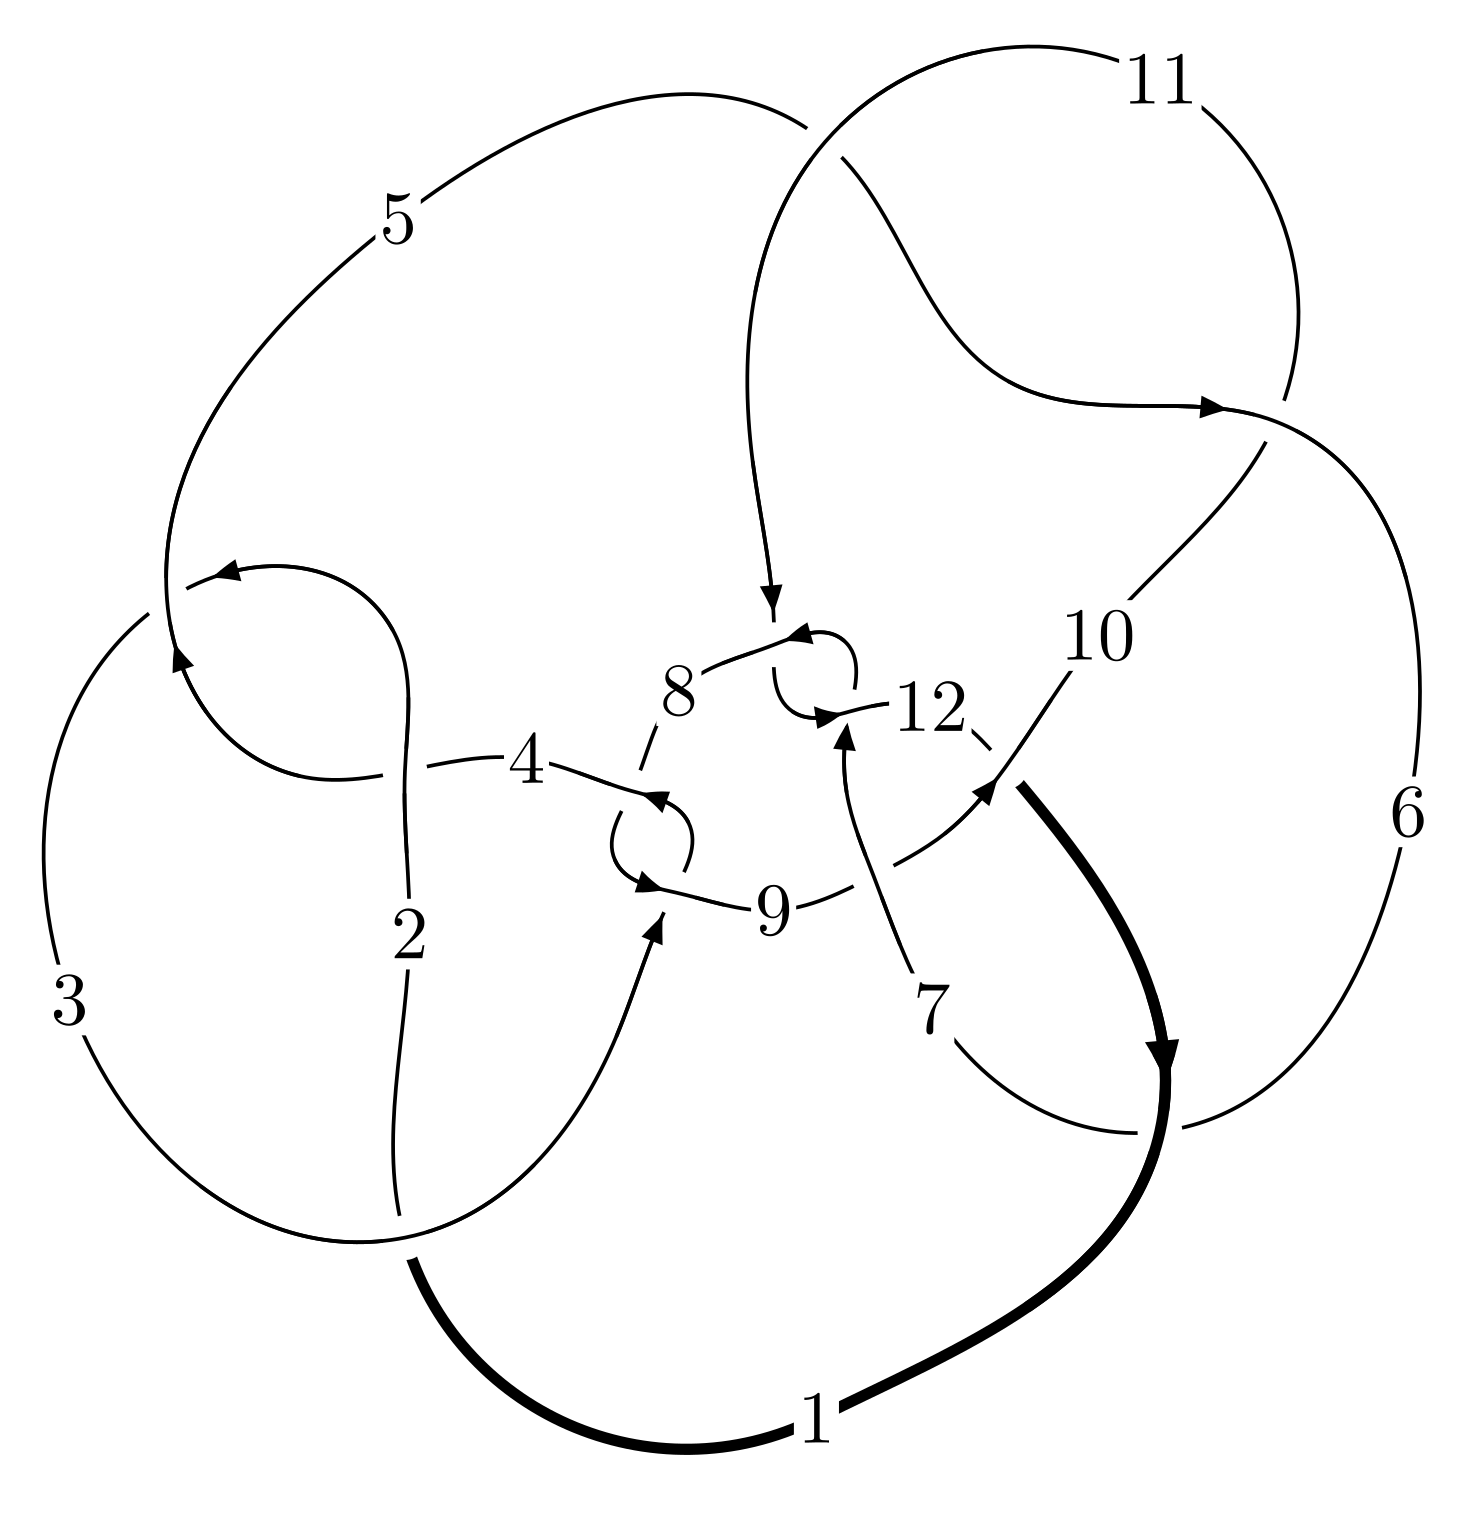
\includegraphics[width=112pt]{../../../GIT/diagram.site/Diagrams/png/964_12a_0163.png}\\
\ \ \ A knot diagram\footnotemark}&
\allowdisplaybreaks
\textbf{Linearized knot diagam} \\
\cline{2-2}
 &
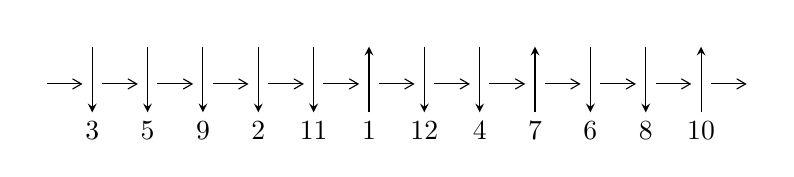
\begin{tikzpicture}[x=20pt, y=17pt]
	% nodes
	\node (C0) at (0, 0) {};
	\node (C1) at (1, 0) {};
	\node (C1U) at (1, +1) {};
	\node (C1D) at (1, -1) {3};

	\node (C2) at (2, 0) {};
	\node (C2U) at (2, +1) {};
	\node (C2D) at (2, -1) {5};

	\node (C3) at (3, 0) {};
	\node (C3U) at (3, +1) {};
	\node (C3D) at (3, -1) {9};

	\node (C4) at (4, 0) {};
	\node (C4U) at (4, +1) {};
	\node (C4D) at (4, -1) {2};

	\node (C5) at (5, 0) {};
	\node (C5U) at (5, +1) {};
	\node (C5D) at (5, -1) {11};

	\node (C6) at (6, 0) {};
	\node (C6U) at (6, +1) {};
	\node (C6D) at (6, -1) {1};

	\node (C7) at (7, 0) {};
	\node (C7U) at (7, +1) {};
	\node (C7D) at (7, -1) {12};

	\node (C8) at (8, 0) {};
	\node (C8U) at (8, +1) {};
	\node (C8D) at (8, -1) {4};

	\node (C9) at (9, 0) {};
	\node (C9U) at (9, +1) {};
	\node (C9D) at (9, -1) {7};

	\node (C10) at (10, 0) {};
	\node (C10U) at (10, +1) {};
	\node (C10D) at (10, -1) {6};

	\node (C11) at (11, 0) {};
	\node (C11U) at (11, +1) {};
	\node (C11D) at (11, -1) {8};

	\node (C12) at (12, 0) {};
	\node (C12U) at (12, +1) {};
	\node (C12D) at (12, -1) {10};
	\node (C13) at (13, 0) {};

	% arrows
	\draw[->,>={angle 60}]
	(C0) edge (C1) (C1) edge (C2) (C2) edge (C3) (C3) edge (C4) (C4) edge (C5) (C5) edge (C6) (C6) edge (C7) (C7) edge (C8) (C8) edge (C9) (C9) edge (C10) (C10) edge (C11) (C11) edge (C12) (C12) edge (C13) ;	\draw[->,>=stealth]
	(C1U) edge (C1D) (C2U) edge (C2D) (C3U) edge (C3D) (C4U) edge (C4D) (C5U) edge (C5D) (C6D) edge (C6U) (C7U) edge (C7D) (C8U) edge (C8D) (C9D) edge (C9U) (C10U) edge (C10D) (C11U) edge (C11D) (C12D) edge (C12U) ;
	\end{tikzpicture} \\
\hhline{~~} \\& 
\textbf{Solving Sequence} \\ \cline{2-2} 
 &
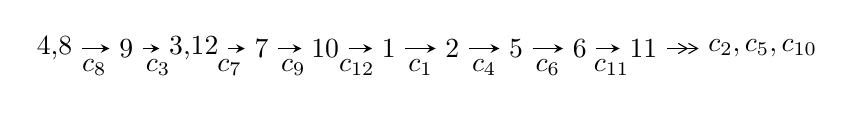
\begin{tikzpicture}[x=23pt, y=7pt]
	% node
	\node (A0) at (-1/8, 0) {4,8};
	\node (A1) at (1, 0) {9};
	\node (A2) at (33/16, 0) {3,12};
	\node (A3) at (25/8, 0) {7};
	\node (A4) at (33/8, 0) {10};
	\node (A5) at (41/8, 0) {1};
	\node (A6) at (49/8, 0) {2};
	\node (A7) at (57/8, 0) {5};
	\node (A8) at (65/8, 0) {6};
	\node (A9) at (73/8, 0) {11};
	\node (C1) at (1/2, -1) {$c_{8}$};
	\node (C2) at (3/2, -1) {$c_{3}$};
	\node (C3) at (21/8, -1) {$c_{7}$};
	\node (C4) at (29/8, -1) {$c_{9}$};
	\node (C5) at (37/8, -1) {$c_{12}$};
	\node (C6) at (45/8, -1) {$c_{1}$};
	\node (C7) at (53/8, -1) {$c_{4}$};
	\node (C8) at (61/8, -1) {$c_{6}$};
	\node (C9) at (69/8, -1) {$c_{11}$};
	\node (A10) at (11, 0) {$c_{2},c_{5},c_{10}$};

	% edge
	\draw[->,>=stealth]	
	(A0) edge (A1) (A1) edge (A2) (A2) edge (A3) (A3) edge (A4) (A4) edge (A5) (A5) edge (A6) (A6) edge (A7) (A7) edge (A8) (A8) edge (A9) ;
	\draw[->>,>={angle 60}]	
	(A9) edge (A10);
\end{tikzpicture} \\ 

\end{tabular} \\

\footnotetext{
The image of knot diagram is generated by the software ``\textbf{Draw programme}" developed by Andrew Bartholomew(\url{http://www.layer8.co.uk/maths/draw/index.htm\#Running-draw}), where we modified some parts for our purpose(\url{https://github.com/CATsTAILs/LinksPainter}).
}\phantom \\ \newline 
\centering \textbf{Ideals for irreducible components\footnotemark of $X_{\text{par}}$} 
 
\begin{align*}
I^u_{1}&=\langle 
2.70227\times10^{92} u^{46}-1.37672\times10^{93} u^{45}+\cdots+1.44449\times10^{95} b+1.08193\times10^{96},\\
\phantom{I^u_{1}}&\phantom{= \langle  }7.39204\times10^{93} u^{46}-4.58246\times10^{94} u^{45}+\cdots+1.15559\times10^{96} a-1.33533\times10^{96},\\
\phantom{I^u_{1}}&\phantom{= \langle  }u^{47}-7 u^{46}+\cdots-3840 u+1024\rangle \\
I^u_{2}&=\langle 
5222 u^6 a^5-8511 u^6 a^4+\cdots+2180 a+5110,\;4 u^6 a^5+36 u^6 a^4+\cdots-226 a+143,\\
\phantom{I^u_{2}}&\phantom{= \langle  }u^7+3 u^6+6 u^5+7 u^4+5 u^3+u^2-2 u-2\rangle \\
I^u_{3}&=\langle 
-17789137958 u^{23}+33220776343 u^{22}+\cdots+123456179965 b+41044745272,\\
\phantom{I^u_{3}}&\phantom{= \langle  }252494650879 u^{23}+77492790641 u^{22}+\cdots+123456179965 a+1483502755409,\\
\phantom{I^u_{3}}&\phantom{= \langle  }u^{24}+6 u^{22}+\cdots+3 u+1\rangle \\
I^u_{4}&=\langle 
-1.70628\times10^{51} a^{11} u^{4}-5.47351\times10^{51} a^{10} u^{4}+\cdots+1.45842\times10^{53} a-6.78636\times10^{52},\\
\phantom{I^u_{4}}&\phantom{= \langle  }-2 a^{11} u^4-3 a^{10} u^4+\cdots-130 a+65,\;u^5- u^4+2 u^3- u^2+u-1\rangle \\
\\
I^v_{1}&=\langle 
a,\;8 v^3+12 v^2+b+10 v+3,\;8 v^4+12 v^3+12 v^2+5 v+1\rangle \\
I^v_{2}&=\langle 
a,\;b^6+b^5+2 b^4+2 b^3+2 b^2+2 b+1,\;v-1\rangle \\
\end{align*}
\raggedright * 6 irreducible components of $\dim_{\mathbb{C}}=0$, with total 183 representations.\\
\footnotetext{All coefficients of polynomials are rational numbers. But the coefficients are sometimes approximated in decimal forms when there is not enough margin.}
\newpage
\renewcommand{\arraystretch}{1}
\centering \section*{I. $I^u_{1}= \langle 2.70\times10^{92} u^{46}-1.38\times10^{93} u^{45}+\cdots+1.44\times10^{95} b+1.08\times10^{96},\;7.39\times10^{93} u^{46}-4.58\times10^{94} u^{45}+\cdots+1.16\times10^{96} a-1.34\times10^{96},\;u^{47}-7 u^{46}+\cdots-3840 u+1024 \rangle$}
\flushleft \textbf{(i) Arc colorings}\\
\begin{tabular}{m{7pt} m{180pt} m{7pt} m{180pt} }
\flushright $a_{4}=$&$\begin{pmatrix}0\\u\end{pmatrix}$ \\
\flushright $a_{8}=$&$\begin{pmatrix}1\\0\end{pmatrix}$ \\
\flushright $a_{9}=$&$\begin{pmatrix}1\\u^2\end{pmatrix}$ \\
\flushright $a_{3}=$&$\begin{pmatrix}u\\u^3+u\end{pmatrix}$ \\
\flushright $a_{12}=$&$\begin{pmatrix}-0.00639675 u^{46}+0.0396546 u^{45}+\cdots-14.8799 u+1.15554\\-0.00187074 u^{46}+0.00953085 u^{45}+\cdots+22.6210 u-7.49001\end{pmatrix}$ \\
\flushright $a_{7}=$&$\begin{pmatrix}-0.0000443720 u^{46}-0.00293863 u^{45}+\cdots+8.66522 u-3.07371\\0.00506215 u^{46}-0.0334217 u^{45}+\cdots+15.5213 u-0.178246\end{pmatrix}$ \\
\flushright $a_{10}=$&$\begin{pmatrix}-0.00734661 u^{46}+0.0494083 u^{45}+\cdots-26.6084 u+6.57684\\-0.00878269 u^{46}+0.0635338 u^{45}+\cdots-64.5424 u+16.8381\end{pmatrix}$ \\
\flushright $a_{1}=$&$\begin{pmatrix}-0.00512383 u^{46}+0.0323413 u^{45}+\cdots-19.6023 u+5.34126\\-0.00609386 u^{46}+0.0454792 u^{45}+\cdots-47.5840 u+16.4994\end{pmatrix}$ \\
\flushright $a_{2}=$&$\begin{pmatrix}-0.00947552 u^{46}+0.0616360 u^{45}+\cdots-36.3597 u+9.72772\\-0.00791514 u^{46}+0.0611719 u^{45}+\cdots-64.3672 u+22.0811\end{pmatrix}$ \\
\flushright $a_{5}=$&$\begin{pmatrix}0.000300958 u^{46}-0.00639035 u^{45}+\cdots+19.6905 u-7.54804\\0.00542479 u^{46}-0.0387317 u^{45}+\cdots+39.2928 u-12.8893\end{pmatrix}$ \\
\flushright $a_{6}=$&$\begin{pmatrix}-0.00471682 u^{46}+0.0299700 u^{45}+\cdots-4.49600 u-3.29609\\0.000362637 u^{46}-0.00530999 u^{45}+\cdots+23.7715 u-12.7111\end{pmatrix}$ \\
\flushright $a_{11}=$&$\begin{pmatrix}-0.00826750 u^{46}+0.0491855 u^{45}+\cdots+7.74105 u-6.33447\\-0.00187074 u^{46}+0.00953085 u^{45}+\cdots+22.6210 u-7.49001\end{pmatrix}$\\&\end{tabular}
\flushleft \textbf{(ii) Obstruction class $= -1$}\\~\\
\flushleft \textbf{(iii) Cusp Shapes $= 0.00835732 u^{46}-0.0282602 u^{45}+\cdots-74.8752 u+42.3285$}\\~\\
\newpage\renewcommand{\arraystretch}{1}
\flushleft \textbf{(iv) u-Polynomials at the component}\newline \\
\begin{tabular}{m{50pt}|m{274pt}}
Crossings & \hspace{64pt}u-Polynomials at each crossing \\
\hline $$\begin{aligned}c_{1}\end{aligned}$$&$\begin{aligned}
&u^{47}+23 u^{46}+\cdots-6912 u+4096
\end{aligned}$\\
\hline $$\begin{aligned}c_{2},c_{4}\end{aligned}$$&$\begin{aligned}
&u^{47}-3 u^{46}+\cdots-240 u+64
\end{aligned}$\\
\hline $$\begin{aligned}c_{3},c_{8}\end{aligned}$$&$\begin{aligned}
&u^{47}-7 u^{46}+\cdots-3840 u+1024
\end{aligned}$\\
\hline $$\begin{aligned}c_{5},c_{7},c_{10}\\c_{11}\end{aligned}$$&$\begin{aligned}
&u^{47}+17 u^{45}+\cdots-2 u+1
\end{aligned}$\\
\hline $$\begin{aligned}c_{6},c_{9}\end{aligned}$$&$\begin{aligned}
&u^{47}+u^{46}+\cdots+5 u+1
\end{aligned}$\\
\hline $$\begin{aligned}c_{12}\end{aligned}$$&$\begin{aligned}
&u^{47}+42 u^{46}+\cdots+3997696 u+131072
\end{aligned}$\\
\hline
\end{tabular}\\~\\
\newpage\renewcommand{\arraystretch}{1}
\flushleft \textbf{(v) Riley Polynomials at the component}\newline \\
\begin{tabular}{m{50pt}|m{274pt}}
Crossings & \hspace{64pt}Riley Polynomials at each crossing \\
\hline $$\begin{aligned}c_{1}\end{aligned}$$&$\begin{aligned}
&y^{47}+5 y^{46}+\cdots+1065680896 y-16777216
\end{aligned}$\\
\hline $$\begin{aligned}c_{2},c_{4}\end{aligned}$$&$\begin{aligned}
&y^{47}-23 y^{46}+\cdots-6912 y-4096
\end{aligned}$\\
\hline $$\begin{aligned}c_{3},c_{8}\end{aligned}$$&$\begin{aligned}
&y^{47}+21 y^{46}+\cdots-11206656 y-1048576
\end{aligned}$\\
\hline $$\begin{aligned}c_{5},c_{7},c_{10}\\c_{11}\end{aligned}$$&$\begin{aligned}
&y^{47}+34 y^{46}+\cdots+22 y-1
\end{aligned}$\\
\hline $$\begin{aligned}c_{6},c_{9}\end{aligned}$$&$\begin{aligned}
&y^{47}+5 y^{46}+\cdots-15 y-1
\end{aligned}$\\
\hline $$\begin{aligned}c_{12}\end{aligned}$$&$\begin{aligned}
&y^{47}-14 y^{46}+\cdots+571230650368 y-17179869184
\end{aligned}$\\
\hline
\end{tabular}\\~\\
\newpage\flushleft \textbf{(vi) Complex Volumes and Cusp Shapes}
$$\begin{array}{c|c|c}  
\text{Solutions to }I^u_{1}& \I (\text{vol} + \sqrt{-1}CS) & \text{Cusp shape}\\
 \hline 
\begin{aligned}
u &= \phantom{-}0.844803 + 0.585454 I \\
a &= \phantom{-}0.382028 - 0.284959 I \\
b &= \phantom{-}0.689635 + 0.097512 I\end{aligned}
 & -3.73817 + 2.80492 I & -12.41752 - 2.95382 I \\ \hline\begin{aligned}
u &= \phantom{-}0.844803 - 0.585454 I \\
a &= \phantom{-}0.382028 + 0.284959 I \\
b &= \phantom{-}0.689635 - 0.097512 I\end{aligned}
 & -3.73817 - 2.80492 I & -12.41752 + 2.95382 I \\ \hline\begin{aligned}
u &= -0.116889 + 1.045570 I \\
a &= \phantom{-}0.478482 - 0.129287 I \\
b &= -0.463355 + 0.003045 I\end{aligned}
 & \phantom{-}2.60054 + 2.28168 I & -2.56476 - 2.68089 I \\ \hline\begin{aligned}
u &= -0.116889 - 1.045570 I \\
a &= \phantom{-}0.478482 + 0.129287 I \\
b &= -0.463355 - 0.003045 I\end{aligned}
 & \phantom{-}2.60054 - 2.28168 I & -2.56476 + 2.68089 I \\ \hline\begin{aligned}
u &= \phantom{-}0.591706 + 0.725415 I \\
a &= \phantom{-}0.318073 + 1.144250 I \\
b &= -0.683715 + 0.183509 I\end{aligned}
 & -4.06475 - 0.35498 I & -12.38504 + 2.03288 I \\ \hline\begin{aligned}
u &= \phantom{-}0.591706 - 0.725415 I \\
a &= \phantom{-}0.318073 - 1.144250 I \\
b &= -0.683715 - 0.183509 I\end{aligned}
 & -4.06475 + 0.35498 I & -12.38504 - 2.03288 I \\ \hline\begin{aligned}
u &= \phantom{-}0.522530 + 0.927802 I \\
a &= \phantom{-}0.377878 - 0.342484 I \\
b &= \phantom{-}0.879419 + 0.351776 I\end{aligned}
 & -3.41339 - 4.10815 I & -9.71270 + 5.53020 I \\ \hline\begin{aligned}
u &= \phantom{-}0.522530 - 0.927802 I \\
a &= \phantom{-}0.377878 + 0.342484 I \\
b &= \phantom{-}0.879419 - 0.351776 I\end{aligned}
 & -3.41339 + 4.10815 I & -9.71270 - 5.53020 I \\ \hline\begin{aligned}
u &= -0.528718 + 0.973805 I \\
a &= \phantom{-}0.234475 - 0.625940 I \\
b &= -0.651818 - 0.000458 I\end{aligned}
 & \phantom{-}0.27510 + 3.56602 I & -7.20697 - 3.60380 I \\ \hline\begin{aligned}
u &= -0.528718 - 0.973805 I \\
a &= \phantom{-}0.234475 + 0.625940 I \\
b &= -0.651818 + 0.000458 I\end{aligned}
 & \phantom{-}0.27510 - 3.56602 I & -7.20697 + 3.60380 I\\
 \hline 
 \end{array}$$\newpage$$\begin{array}{c|c|c}  
\text{Solutions to }I^u_{1}& \I (\text{vol} + \sqrt{-1}CS) & \text{Cusp shape}\\
 \hline 
\begin{aligned}
u &= -0.378274 + 1.041930 I \\
a &= \phantom{-}0.55552 + 1.57805 I \\
b &= -0.164802 - 0.759470 I\end{aligned}
 & -1.01111 - 1.34745 I & -8.38291 - 3.53586 I \\ \hline\begin{aligned}
u &= -0.378274 - 1.041930 I \\
a &= \phantom{-}0.55552 - 1.57805 I \\
b &= -0.164802 + 0.759470 I\end{aligned}
 & -1.01111 + 1.34745 I & -8.38291 + 3.53586 I \\ \hline\begin{aligned}
u &= \phantom{-}0.806009 + 0.772506 I \\
a &= -0.251056 + 0.347370 I \\
b &= -0.286940 - 0.929982 I\end{aligned}
 & -0.81815 - 8.32208 I & -3.76133 + 11.43016 I \\ \hline\begin{aligned}
u &= \phantom{-}0.806009 - 0.772506 I \\
a &= -0.251056 - 0.347370 I \\
b &= -0.286940 + 0.929982 I\end{aligned}
 & -0.81815 + 8.32208 I & -3.76133 - 11.43016 I \\ \hline\begin{aligned}
u &= \phantom{-}0.364619 + 1.136610 I \\
a &= \phantom{-}0.68230 - 2.35146 I \\
b &= \phantom{-}0.50792 + 1.37152 I\end{aligned}
 & \phantom{-}3.40359 - 9.98566 I & -2.62320 + 6.71929 I \\ \hline\begin{aligned}
u &= \phantom{-}0.364619 - 1.136610 I \\
a &= \phantom{-}0.68230 + 2.35146 I \\
b &= \phantom{-}0.50792 - 1.37152 I\end{aligned}
 & \phantom{-}3.40359 + 9.98566 I & -2.62320 - 6.71929 I \\ \hline\begin{aligned}
u &= -1.203240 + 0.185614 I \\
a &= -0.141165 + 0.382761 I \\
b &= -0.43658 - 1.36501 I\end{aligned}
 & \phantom{-}5.86998 - 7.58123 I & -1.27065 + 3.88153 I \\ \hline\begin{aligned}
u &= -1.203240 - 0.185614 I \\
a &= -0.141165 - 0.382761 I \\
b &= -0.43658 + 1.36501 I\end{aligned}
 & \phantom{-}5.86998 + 7.58123 I & -1.27065 - 3.88153 I \\ \hline\begin{aligned}
u &= \phantom{-}0.658190 + 1.049420 I \\
a &= \phantom{-}0.023470 + 0.617425 I \\
b &= -0.763224 - 0.063672 I\end{aligned}
 & -2.27485 - 8.39804 I & -10.61831 + 8.01791 I \\ \hline\begin{aligned}
u &= \phantom{-}0.658190 - 1.049420 I \\
a &= \phantom{-}0.023470 - 0.617425 I \\
b &= -0.763224 + 0.063672 I\end{aligned}
 & -2.27485 + 8.39804 I & -10.61831 - 8.01791 I\\
 \hline 
 \end{array}$$\newpage$$\begin{array}{c|c|c}  
\text{Solutions to }I^u_{1}& \I (\text{vol} + \sqrt{-1}CS) & \text{Cusp shape}\\
 \hline 
\begin{aligned}
u &= \phantom{-}0.117325 + 0.702557 I \\
a &= \phantom{-}0.366852 + 0.421918 I \\
b &= \phantom{-}0.708072 - 0.641224 I\end{aligned}
 & -1.83722 + 0.84307 I & -4.20177 + 0.72689 I \\ \hline\begin{aligned}
u &= \phantom{-}0.117325 - 0.702557 I \\
a &= \phantom{-}0.366852 - 0.421918 I \\
b &= \phantom{-}0.708072 + 0.641224 I\end{aligned}
 & -1.83722 - 0.84307 I & -4.20177 - 0.72689 I \\ \hline\begin{aligned}
u &= \phantom{-}1.194080 + 0.493935 I \\
a &= -0.138037 - 0.364269 I \\
b &= -0.54468 + 1.40917 I\end{aligned}
 & \phantom{-}4.46440 + 12.91220 I & -3.19580 - 7.97672 I \\ \hline\begin{aligned}
u &= \phantom{-}1.194080 - 0.493935 I \\
a &= -0.138037 + 0.364269 I \\
b &= -0.54468 - 1.40917 I\end{aligned}
 & \phantom{-}4.46440 - 12.91220 I & -3.19580 + 7.97672 I \\ \hline\begin{aligned}
u &= -0.529603 + 0.452776 I \\
a &= \phantom{-}0.463480 + 0.338892 I \\
b &= \phantom{-}0.572558 - 0.322699 I\end{aligned}
 & -1.134430 + 0.669866 I & -7.99633 - 3.35670 I \\ \hline\begin{aligned}
u &= -0.529603 - 0.452776 I \\
a &= \phantom{-}0.463480 - 0.338892 I \\
b &= \phantom{-}0.572558 + 0.322699 I\end{aligned}
 & -1.134430 - 0.669866 I & -7.99633 + 3.35670 I \\ \hline\begin{aligned}
u &= -0.593581\phantom{ +0.000000I} \\
a &= \phantom{-}0.650414\phantom{ +0.000000I} \\
b &= \phantom{-}0.304199\phantom{ +0.000000I}\end{aligned}
 & -1.03435\phantom{ +0.000000I} & -10.4580\phantom{ +0.000000I} \\ \hline\begin{aligned}
u &= \phantom{-}0.230767 + 0.543413 I \\
a &= -0.171169 - 0.354083 I \\
b &= -0.618665 + 1.130340 I\end{aligned}
 & \phantom{-}1.16202 + 7.20671 I & \phantom{-}1.21848 + 2.56039 I \\ \hline\begin{aligned}
u &= \phantom{-}0.230767 - 0.543413 I \\
a &= -0.171169 + 0.354083 I \\
b &= -0.618665 - 1.130340 I\end{aligned}
 & \phantom{-}1.16202 - 7.20671 I & \phantom{-}1.21848 - 2.56039 I \\ \hline\begin{aligned}
u &= \phantom{-}1.41557 + 0.19018 I \\
a &= \phantom{-}0.238371 + 0.686766 I \\
b &= \phantom{-}0.267051 - 0.946782 I\end{aligned}
 & \phantom{-}1.14395 + 4.11529 I & \phantom{-0.000000 } 0. - 15.1609 I\\
 \hline 
 \end{array}$$\newpage$$\begin{array}{c|c|c}  
\text{Solutions to }I^u_{1}& \I (\text{vol} + \sqrt{-1}CS) & \text{Cusp shape}\\
 \hline 
\begin{aligned}
u &= \phantom{-}1.41557 - 0.19018 I \\
a &= \phantom{-}0.238371 - 0.686766 I \\
b &= \phantom{-}0.267051 + 0.946782 I\end{aligned}
 & \phantom{-}1.14395 - 4.11529 I & \phantom{-0.000000 -}0. + 15.1609 I \\ \hline\begin{aligned}
u &= -1.22540 + 0.75189 I \\
a &= -0.246090 - 0.506658 I \\
b &= -0.113298 + 1.119510 I\end{aligned}
 & \phantom{-}3.81471 + 4.15254 I & \phantom{-0.000000 } 0 \\ \hline\begin{aligned}
u &= -1.22540 - 0.75189 I \\
a &= -0.246090 + 0.506658 I \\
b &= -0.113298 - 1.119510 I\end{aligned}
 & \phantom{-}3.81471 - 4.15254 I & \phantom{-0.000000 } 0 \\ \hline\begin{aligned}
u &= -0.60695 + 1.32433 I \\
a &= \phantom{-}0.83079 + 1.66964 I \\
b &= \phantom{-}0.56919 - 1.47090 I\end{aligned}
 & \phantom{-}9.5566 + 13.8984 I & \phantom{-0.000000 } 0 \\ \hline\begin{aligned}
u &= -0.60695 - 1.32433 I \\
a &= \phantom{-}0.83079 - 1.66964 I \\
b &= \phantom{-}0.56919 + 1.47090 I\end{aligned}
 & \phantom{-}9.5566 - 13.8984 I & \phantom{-0.000000 } 0 \\ \hline\begin{aligned}
u &= \phantom{-}0.75973 + 1.26376 I \\
a &= \phantom{-}1.05216 - 1.49784 I \\
b &= \phantom{-}0.63326 + 1.46597 I\end{aligned}
 & \phantom{-}6.9588 - 19.8841 I & \phantom{-0.000000 } 0 \\ \hline\begin{aligned}
u &= \phantom{-}0.75973 - 1.26376 I \\
a &= \phantom{-}1.05216 + 1.49784 I \\
b &= \phantom{-}0.63326 - 1.46597 I\end{aligned}
 & \phantom{-}6.9588 + 19.8841 I & \phantom{-0.000000 } 0 \\ \hline\begin{aligned}
u &= \phantom{-}0.99117 + 1.12526 I \\
a &= -0.548310 + 0.653114 I \\
b &= \phantom{-}0.034489 - 1.053340 I\end{aligned}
 & \phantom{-}0.02289 + 1.75896 I & \phantom{-0.000000 } 0 \\ \hline\begin{aligned}
u &= \phantom{-}0.99117 - 1.12526 I \\
a &= -0.548310 - 0.653114 I \\
b &= \phantom{-}0.034489 + 1.053340 I\end{aligned}
 & \phantom{-}0.02289 - 1.75896 I & \phantom{-0.000000 } 0 \\ \hline\begin{aligned}
u &= -0.00707 + 1.54573 I \\
a &= -0.12787 + 1.62424 I \\
b &= \phantom{-}0.30210 - 1.45757 I\end{aligned}
 & \phantom{-}12.5387 + 8.5475 I & \phantom{-0.000000 } 0\\
 \hline 
 \end{array}$$\newpage$$\begin{array}{c|c|c}  
\text{Solutions to }I^u_{1}& \I (\text{vol} + \sqrt{-1}CS) & \text{Cusp shape}\\
 \hline 
\begin{aligned}
u &= -0.00707 - 1.54573 I \\
a &= -0.12787 - 1.62424 I \\
b &= \phantom{-}0.30210 + 1.45757 I\end{aligned}
 & \phantom{-}12.5387 - 8.5475 I & \phantom{-0.000000 } 0 \\ \hline\begin{aligned}
u &= \phantom{-}0.75783 + 1.35531 I \\
a &= -0.77762 + 1.33679 I \\
b &= -0.448938 - 1.118610 I\end{aligned}
 & \phantom{-}4.59247 - 11.54410 I & \phantom{-0.000000 } 0 \\ \hline\begin{aligned}
u &= \phantom{-}0.75783 - 1.35531 I \\
a &= -0.77762 - 1.33679 I \\
b &= -0.448938 + 1.118610 I\end{aligned}
 & \phantom{-}4.59247 + 11.54410 I & \phantom{-0.000000 } 0 \\ \hline\begin{aligned}
u &= -0.25517 + 1.56898 I \\
a &= -0.38203 - 1.44288 I \\
b &= \phantom{-}0.18549 + 1.40391 I\end{aligned}
 & \phantom{-}12.10480 - 1.94711 I & \phantom{-0.000000 } 0 \\ \hline\begin{aligned}
u &= -0.25517 - 1.56898 I \\
a &= -0.38203 + 1.44288 I \\
b &= \phantom{-}0.18549 - 1.40391 I\end{aligned}
 & \phantom{-}12.10480 + 1.94711 I & \phantom{-0.000000 } 0 \\ \hline\begin{aligned}
u &= -0.60622 + 1.51689 I \\
a &= -0.54574 - 1.36308 I \\
b &= -0.325270 + 1.113800 I\end{aligned}
 & \phantom{-}7.05094 + 5.09408 I & \phantom{-0.000000 } 0 \\ \hline\begin{aligned}
u &= -0.60622 - 1.51689 I \\
a &= -0.54574 + 1.36308 I \\
b &= -0.325270 - 1.113800 I\end{aligned}
 & \phantom{-}7.05094 - 5.09408 I & \phantom{-0.000000 } 0\\
 \hline 
 \end{array}$$\newpage\newpage\renewcommand{\arraystretch}{1}
\centering \section*{II. $I^u_{2}= \langle 5222 u^6 a^5-8511 u^6 a^4+\cdots+2180 a+5110,\;4 u^6 a^5+36 u^6 a^4+\cdots-226 a+143,\;u^7+3 u^6+6 u^5+7 u^4+5 u^3+u^2-2 u-2 \rangle$}
\flushleft \textbf{(i) Arc colorings}\\
\begin{tabular}{m{7pt} m{180pt} m{7pt} m{180pt} }
\flushright $a_{4}=$&$\begin{pmatrix}0\\u\end{pmatrix}$ \\
\flushright $a_{8}=$&$\begin{pmatrix}1\\0\end{pmatrix}$ \\
\flushright $a_{9}=$&$\begin{pmatrix}1\\u^2\end{pmatrix}$ \\
\flushright $a_{3}=$&$\begin{pmatrix}u\\u^3+u\end{pmatrix}$ \\
\flushright $a_{12}=$&$\begin{pmatrix}a\\-1.16329 a^{5} u^{6}+1.89597 a^{4} u^{6}+\cdots-0.485632 a-1.13834\end{pmatrix}$ \\
\flushright $a_{7}=$&$\begin{pmatrix}1.14881 a^{5} u^{6}-2.32880 a^{4} u^{6}+\cdots-0.264647 a-2.56315\\1.40031 a^{5} u^{6}-1.46536 a^{4} u^{6}+\cdots+5.84495 a-0.453553\end{pmatrix}$ \\
\flushright $a_{10}=$&$\begin{pmatrix}1.28403 a^{4} u^{6}-0.761194 a^{3} u^{6}+\cdots+0.298507 a+3.07062\\0.806416 a^{4} u^{6}+0.432836 a^{3} u^{6}+\cdots-4.20896 a-0.630875\end{pmatrix}$ \\
\flushright $a_{1}=$&$\begin{pmatrix}-\frac{1}{2} u^6-\frac{3}{2} u^5+\cdots-\frac{1}{2} u^2+\frac{1}{2} u\\u^6+2 u^5+3 u^4+2 u^3- u-1\end{pmatrix}$ \\
\flushright $a_{2}=$&$\begin{pmatrix}-\frac{1}{2} u^6-\frac{1}{2} u^5+\cdots-\frac{1}{2} u^2-\frac{1}{2} u\\- u^6-2 u^5-3 u^4-3 u^3- u^2+1\end{pmatrix}$ \\
\flushright $a_{5}=$&$\begin{pmatrix}-\frac{1}{2} u^6-\frac{3}{2} u^5+\cdots+\frac{1}{2} u+1\\- u^4- u^3- u^2+1\end{pmatrix}$ \\
\flushright $a_{6}=$&$\begin{pmatrix}1.55358 a^{5} u^{6}-3.01359 a^{4} u^{6}+\cdots+1.79394 a-1.80307\\0.747160 a^{5} u^{6}-2.29762 a^{4} u^{6}+\cdots+1.12631 a+0.230786\end{pmatrix}$ \\
\flushright $a_{11}=$&$\begin{pmatrix}-1.16329 a^{5} u^{6}+1.89597 a^{4} u^{6}+\cdots+0.514368 a-1.13834\\-1.16329 a^{5} u^{6}+1.89597 a^{4} u^{6}+\cdots-0.485632 a-1.13834\end{pmatrix}$\\&\end{tabular}
\flushleft \textbf{(ii) Obstruction class $= -1$}\\~\\
\flushleft \textbf{(iii) Cusp Shapes $= -\frac{20628}{4489} u^6 a^4+\frac{280}{67} u^6 a^3+\cdots-\frac{320}{67} a-\frac{18564}{4489}$}\\~\\
\newpage\renewcommand{\arraystretch}{1}
\flushleft \textbf{(iv) u-Polynomials at the component}\newline \\
\begin{tabular}{m{50pt}|m{274pt}}
Crossings & \hspace{64pt}u-Polynomials at each crossing \\
\hline $$\begin{aligned}c_{1}\end{aligned}$$&$\begin{aligned}
&(u^7+3 u^6+7 u^5+8 u^4+9 u^3+6 u^2+5 u+1)^6
\end{aligned}$\\
\hline $$\begin{aligned}c_{2},c_{4}\end{aligned}$$&$\begin{aligned}
&(u^7- u^6- u^5+2 u^4+u^3-2 u^2+u+1)^6
\end{aligned}$\\
\hline $$\begin{aligned}c_{3},c_{8}\end{aligned}$$&$\begin{aligned}
&(u^7+3 u^6+6 u^5+7 u^4+5 u^3+u^2-2 u-2)^6
\end{aligned}$\\
\hline $$\begin{aligned}c_{5},c_{7},c_{10}\\c_{11}\end{aligned}$$&$\begin{aligned}
&u^{42}+u^{41}+\cdots-1560 u+347
\end{aligned}$\\
\hline $$\begin{aligned}c_{6},c_{9}\end{aligned}$$&$\begin{aligned}
&u^{42}+3 u^{41}+\cdots+130 u+53
\end{aligned}$\\
\hline $$\begin{aligned}c_{12}\end{aligned}$$&$\begin{aligned}
&(u^3- u^2+1)^{14}
\end{aligned}$\\
\hline
\end{tabular}\\~\\
\newpage\renewcommand{\arraystretch}{1}
\flushleft \textbf{(v) Riley Polynomials at the component}\newline \\
\begin{tabular}{m{50pt}|m{274pt}}
Crossings & \hspace{64pt}Riley Polynomials at each crossing \\
\hline $$\begin{aligned}c_{1}\end{aligned}$$&$\begin{aligned}
&(y^7+5 y^6+19 y^5+36 y^4+49 y^3+38 y^2+13 y-1)^6
\end{aligned}$\\
\hline $$\begin{aligned}c_{2},c_{4}\end{aligned}$$&$\begin{aligned}
&(y^7-3 y^6+7 y^5-8 y^4+9 y^3-6 y^2+5 y-1)^6
\end{aligned}$\\
\hline $$\begin{aligned}c_{3},c_{8}\end{aligned}$$&$\begin{aligned}
&(y^7+3 y^6+4 y^5+y^4- y^3+7 y^2+8 y-4)^6
\end{aligned}$\\
\hline $$\begin{aligned}c_{5},c_{7},c_{10}\\c_{11}\end{aligned}$$&$\begin{aligned}
&y^{42}+33 y^{41}+\cdots+486752 y+120409
\end{aligned}$\\
\hline $$\begin{aligned}c_{6},c_{9}\end{aligned}$$&$\begin{aligned}
&y^{42}-11 y^{41}+\cdots-87496 y+2809
\end{aligned}$\\
\hline $$\begin{aligned}c_{12}\end{aligned}$$&$\begin{aligned}
&(y^3- y^2+2 y-1)^{14}
\end{aligned}$\\
\hline
\end{tabular}\\~\\
\newpage\flushleft \textbf{(vi) Complex Volumes and Cusp Shapes}
$$\begin{array}{c|c|c}  
\text{Solutions to }I^u_{2}& \I (\text{vol} + \sqrt{-1}CS) & \text{Cusp shape}\\
 \hline 
\begin{aligned}
u &= -0.984140 + 0.426152 I \\
a &= \phantom{-}0.737720 + 0.711168 I \\
b &= \phantom{-}0.418947 - 0.385328 I\end{aligned}
 & -0.184741 - 1.102580 I & -5.76916 + 1.89286 I \\ \hline\begin{aligned}
u &= -0.984140 + 0.426152 I \\
a &= -0.793584 - 0.796489 I \\
b &= -1.239540 - 0.061605 I\end{aligned}
 & -0.18474 - 6.75882 I & -5.76916 + 7.85175 I \\ \hline\begin{aligned}
u &= -0.984140 + 0.426152 I \\
a &= \phantom{-}0.841475 + 0.111964 I \\
b &= \phantom{-}0.130488 + 1.167740 I\end{aligned}
 & \phantom{-}3.95284 - 3.93070 I & \phantom{-}0.76010 + 4.87230 I \\ \hline\begin{aligned}
u &= -0.984140 + 0.426152 I \\
a &= \phantom{-}0.116149 - 0.835603 I \\
b &= \phantom{-}0.365594 + 1.240650 I\end{aligned}
 & -0.18474 - 6.75882 I & -5.76916 + 7.85175 I \\ \hline\begin{aligned}
u &= -0.984140 + 0.426152 I \\
a &= \phantom{-}0.426938 + 0.617821 I \\
b &= \phantom{-}0.031150 - 1.011580 I\end{aligned}
 & -0.184741 - 1.102580 I & -5.76916 + 1.89286 I \\ \hline\begin{aligned}
u &= -0.984140 + 0.426152 I \\
a &= -0.196042 - 0.513489 I \\
b &= -0.69197 - 1.45635 I\end{aligned}
 & \phantom{-}3.95284 - 3.93070 I & \phantom{-}0.76010 + 4.87230 I \\ \hline\begin{aligned}
u &= -0.984140 - 0.426152 I \\
a &= \phantom{-}0.737720 - 0.711168 I \\
b &= \phantom{-}0.418947 + 0.385328 I\end{aligned}
 & -0.184741 + 1.102580 I & -5.76916 - 1.89286 I \\ \hline\begin{aligned}
u &= -0.984140 - 0.426152 I \\
a &= -0.793584 + 0.796489 I \\
b &= -1.239540 + 0.061605 I\end{aligned}
 & -0.18474 + 6.75882 I & -5.76916 - 7.85175 I \\ \hline\begin{aligned}
u &= -0.984140 - 0.426152 I \\
a &= \phantom{-}0.841475 - 0.111964 I \\
b &= \phantom{-}0.130488 - 1.167740 I\end{aligned}
 & \phantom{-}3.95284 + 3.93070 I & \phantom{-}0.76010 - 4.87230 I \\ \hline\begin{aligned}
u &= -0.984140 - 0.426152 I \\
a &= \phantom{-}0.116149 + 0.835603 I \\
b &= \phantom{-}0.365594 - 1.240650 I\end{aligned}
 & -0.18474 + 6.75882 I & -5.76916 - 7.85175 I\\
 \hline 
 \end{array}$$\newpage$$\begin{array}{c|c|c}  
\text{Solutions to }I^u_{2}& \I (\text{vol} + \sqrt{-1}CS) & \text{Cusp shape}\\
 \hline 
\begin{aligned}
u &= -0.984140 - 0.426152 I \\
a &= \phantom{-}0.426938 - 0.617821 I \\
b &= \phantom{-}0.031150 + 1.011580 I\end{aligned}
 & -0.184741 + 1.102580 I & -5.76916 - 1.89286 I \\ \hline\begin{aligned}
u &= -0.984140 - 0.426152 I \\
a &= -0.196042 + 0.513489 I \\
b &= -0.69197 + 1.45635 I\end{aligned}
 & \phantom{-}3.95284 + 3.93070 I & \phantom{-}0.76010 - 4.87230 I \\ \hline\begin{aligned}
u &= -0.167785 + 1.218780 I \\
a &= -0.788443 - 0.203769 I \\
b &= -0.405655 - 0.307642 I\end{aligned}
 & \phantom{-}5.76303 + 1.87273 I & \phantom{-}1.179538 - 0.608619 I \\ \hline\begin{aligned}
u &= -0.167785 + 1.218780 I \\
a &= -0.363766 + 0.081288 I \\
b &= \phantom{-}1.218000 + 0.569803 I\end{aligned}
 & \phantom{-}5.76303 - 3.78352 I & \phantom{-}1.17954 + 5.35027 I \\ \hline\begin{aligned}
u &= -0.167785 + 1.218780 I \\
a &= -0.52032 - 1.78091 I \\
b &= \phantom{-}0.47547 + 1.85744 I\end{aligned}
 & \phantom{-}9.90062 - 0.95540 I & \phantom{-}7.70880 + 2.37083 I \\ \hline\begin{aligned}
u &= -0.167785 + 1.218780 I \\
a &= -0.38206 - 1.99236 I \\
b &= -0.477401 + 1.254840 I\end{aligned}
 & \phantom{-}5.76303 + 1.87273 I & \phantom{-}1.179538 - 0.608619 I \\ \hline\begin{aligned}
u &= -0.167785 + 1.218780 I \\
a &= -0.49358 + 2.12435 I \\
b &= -0.13510 - 1.41647 I\end{aligned}
 & \phantom{-}9.90062 - 0.95540 I & \phantom{-}7.70880 + 2.37083 I \\ \hline\begin{aligned}
u &= -0.167785 + 1.218780 I \\
a &= \phantom{-}0.76890 + 2.37410 I \\
b &= -0.078011 - 1.184130 I\end{aligned}
 & \phantom{-}5.76303 - 3.78352 I & \phantom{-}1.17954 + 5.35027 I \\ \hline\begin{aligned}
u &= -0.167785 - 1.218780 I \\
a &= -0.788443 + 0.203769 I \\
b &= -0.405655 + 0.307642 I\end{aligned}
 & \phantom{-}5.76303 - 1.87273 I & \phantom{-}1.179538 + 0.608619 I \\ \hline\begin{aligned}
u &= -0.167785 - 1.218780 I \\
a &= -0.363766 - 0.081288 I \\
b &= \phantom{-}1.218000 - 0.569803 I\end{aligned}
 & \phantom{-}5.76303 + 3.78352 I & \phantom{-}1.17954 - 5.35027 I\\
 \hline 
 \end{array}$$\newpage$$\begin{array}{c|c|c}  
\text{Solutions to }I^u_{2}& \I (\text{vol} + \sqrt{-1}CS) & \text{Cusp shape}\\
 \hline 
\begin{aligned}
u &= -0.167785 - 1.218780 I \\
a &= -0.52032 + 1.78091 I \\
b &= \phantom{-}0.47547 - 1.85744 I\end{aligned}
 & \phantom{-}9.90062 + 0.95540 I & \phantom{-}7.70880 - 2.37083 I \\ \hline\begin{aligned}
u &= -0.167785 - 1.218780 I \\
a &= -0.38206 + 1.99236 I \\
b &= -0.477401 - 1.254840 I\end{aligned}
 & \phantom{-}5.76303 - 1.87273 I & \phantom{-}1.179538 + 0.608619 I \\ \hline\begin{aligned}
u &= -0.167785 - 1.218780 I \\
a &= -0.49358 - 2.12435 I \\
b &= -0.13510 + 1.41647 I\end{aligned}
 & \phantom{-}9.90062 + 0.95540 I & \phantom{-}7.70880 - 2.37083 I \\ \hline\begin{aligned}
u &= -0.167785 - 1.218780 I \\
a &= \phantom{-}0.76890 - 2.37410 I \\
b &= -0.078011 + 1.184130 I\end{aligned}
 & \phantom{-}5.76303 + 3.78352 I & \phantom{-}1.17954 - 5.35027 I \\ \hline\begin{aligned}
u &= -0.654547 + 1.202470 I \\
a &= -0.141241 + 0.714180 I \\
b &= \phantom{-}1.46294 - 0.00954 I\end{aligned}
 & \phantom{-}2.27436 + 12.75880 I & -3.97003 - 10.31609 I \\ \hline\begin{aligned}
u &= -0.654547 + 1.202470 I \\
a &= \phantom{-}0.76606 + 1.40096 I \\
b &= \phantom{-}0.152871 - 1.268940 I\end{aligned}
 & \phantom{-}2.27436 + 7.10253 I & -3.97003 - 4.35720 I \\ \hline\begin{aligned}
u &= -0.654547 + 1.202470 I \\
a &= \phantom{-}1.00141 + 1.33815 I \\
b &= \phantom{-}0.91938 - 1.48492 I\end{aligned}
 & \phantom{-}6.41195 + 9.93065 I & \phantom{-}2.55923 - 7.33664 I \\ \hline\begin{aligned}
u &= -0.654547 + 1.202470 I \\
a &= -1.57657 - 0.89969 I \\
b &= -0.270073 + 1.125830 I\end{aligned}
 & \phantom{-}6.41195 + 9.93065 I & \phantom{-}2.55923 - 7.33664 I \\ \hline\begin{aligned}
u &= -0.654547 + 1.202470 I \\
a &= \phantom{-}0.0226124 + 0.0838717 I \\
b &= -0.731518 - 0.356031 I\end{aligned}
 & \phantom{-}2.27436 + 7.10253 I & -3.97003 - 4.35720 I \\ \hline\begin{aligned}
u &= -0.654547 + 1.202470 I \\
a &= -1.08160 - 1.86803 I \\
b &= -0.39415 + 1.36343 I\end{aligned}
 & \phantom{-}2.27436 + 12.75880 I & -3.97003 - 10.31609 I\\
 \hline 
 \end{array}$$\newpage$$\begin{array}{c|c|c}  
\text{Solutions to }I^u_{2}& \I (\text{vol} + \sqrt{-1}CS) & \text{Cusp shape}\\
 \hline 
\begin{aligned}
u &= -0.654547 - 1.202470 I \\
a &= -0.141241 - 0.714180 I \\
b &= \phantom{-}1.46294 + 0.00954 I\end{aligned}
 & \phantom{-}2.27436 - 12.75880 I & -3.97003 + 10.31609 I \\ \hline\begin{aligned}
u &= -0.654547 - 1.202470 I \\
a &= \phantom{-}0.76606 - 1.40096 I \\
b &= \phantom{-}0.152871 + 1.268940 I\end{aligned}
 & \phantom{-}2.27436 - 7.10253 I & -3.97003 + 4.35720 I \\ \hline\begin{aligned}
u &= -0.654547 - 1.202470 I \\
a &= \phantom{-}1.00141 - 1.33815 I \\
b &= \phantom{-}0.91938 + 1.48492 I\end{aligned}
 & \phantom{-}6.41195 - 9.93065 I & \phantom{-}2.55923 + 7.33664 I \\ \hline\begin{aligned}
u &= -0.654547 - 1.202470 I \\
a &= -1.57657 + 0.89969 I \\
b &= -0.270073 - 1.125830 I\end{aligned}
 & \phantom{-}6.41195 - 9.93065 I & \phantom{-}2.55923 + 7.33664 I \\ \hline\begin{aligned}
u &= -0.654547 - 1.202470 I \\
a &= \phantom{-}0.0226124 - 0.0838717 I \\
b &= -0.731518 + 0.356031 I\end{aligned}
 & \phantom{-}2.27436 - 7.10253 I & -3.97003 + 4.35720 I \\ \hline\begin{aligned}
u &= -0.654547 - 1.202470 I \\
a &= -1.08160 + 1.86803 I \\
b &= -0.39415 - 1.36343 I\end{aligned}
 & \phantom{-}2.27436 - 12.75880 I & -3.97003 + 10.31609 I \\ \hline\begin{aligned}
u &= \phantom{-}0.612945\phantom{ +0.000000I} \\
a &= \phantom{-}0.92534 + 1.35436 I \\
b &= \phantom{-}0.376065 - 0.940931 I\end{aligned}
 & \phantom{-}0.95928 + 2.82812 I & -5.44897 - 2.97945 I \\ \hline\begin{aligned}
u &= \phantom{-}0.612945\phantom{ +0.000000I} \\
a &= \phantom{-}0.92534 - 1.35436 I \\
b &= \phantom{-}0.376065 + 0.940931 I\end{aligned}
 & \phantom{-}0.95928 - 2.82812 I & -5.44897 + 2.97945 I \\ \hline\begin{aligned}
u &= \phantom{-}0.612945\phantom{ +0.000000I} \\
a &= \phantom{-}0.94362 + 1.89521 I \\
b &= -0.14327 + 1.43225 I\end{aligned}
 & \phantom{-}5.09686\phantom{ +0.000000I} & \phantom{-}                -6
1.080296 + 0. 10   I\phantom{ +0.000000I} \\ \hline\begin{aligned}
u &= \phantom{-}0.612945\phantom{ +0.000000I} \\
a &= \phantom{-}0.94362 - 1.89521 I \\
b &= -0.14327 - 1.43225 I\end{aligned}
 & \phantom{-}5.09686\phantom{ +0.000000I} & \phantom{-}                -6
1.080296 + 0. 10   I\phantom{ +0.000000I}\\
 \hline 
 \end{array}$$\newpage$$\begin{array}{c|c|c}  
\text{Solutions to }I^u_{2}& \I (\text{vol} + \sqrt{-1}CS) & \text{Cusp shape}\\
 \hline 
\begin{aligned}
u &= \phantom{-}0.612945\phantom{ +0.000000I} \\
a &= -0.21302 + 2.97475 I \\
b &= -0.484219 + 0.283629 I\end{aligned}
 & \phantom{-}0.95928 + 2.82812 I & -5.44897 - 2.97945 I \\ \hline\begin{aligned}
u &= \phantom{-}0.612945\phantom{ +0.000000I} \\
a &= -0.21302 - 2.97475 I \\
b &= -0.484219 - 0.283629 I\end{aligned}
 & \phantom{-}0.95928 - 2.82812 I & -5.44897 + 2.97945 I\\
 \hline 
 \end{array}$$\newpage\newpage\renewcommand{\arraystretch}{1}
\centering \section*{III. $I^u_{3}= \langle -1.78\times10^{10} u^{23}+3.32\times10^{10} u^{22}+\cdots+1.23\times10^{11} b+4.10\times10^{10},\;2.52\times10^{11} u^{23}+7.75\times10^{10} u^{22}+\cdots+1.23\times10^{11} a+1.48\times10^{12},\;u^{24}+6 u^{22}+\cdots+3 u+1 \rangle$}
\flushleft \textbf{(i) Arc colorings}\\
\begin{tabular}{m{7pt} m{180pt} m{7pt} m{180pt} }
\flushright $a_{4}=$&$\begin{pmatrix}0\\u\end{pmatrix}$ \\
\flushright $a_{8}=$&$\begin{pmatrix}1\\0\end{pmatrix}$ \\
\flushright $a_{9}=$&$\begin{pmatrix}1\\u^2\end{pmatrix}$ \\
\flushright $a_{3}=$&$\begin{pmatrix}u\\u^3+u\end{pmatrix}$ \\
\flushright $a_{12}=$&$\begin{pmatrix}-2.04522 u^{23}-0.627695 u^{22}+\cdots-0.358592 u-12.0164\\0.144093 u^{23}-0.269090 u^{22}+\cdots+0.758652 u-0.332464\end{pmatrix}$ \\
\flushright $a_{7}=$&$\begin{pmatrix}2.81971 u^{23}-2.21363 u^{22}+\cdots+17.5956 u+1.17885\\0.135846 u^{23}-0.0946331 u^{22}+\cdots+1.96665 u+0.813872\end{pmatrix}$ \\
\flushright $a_{10}=$&$\begin{pmatrix}2.91642 u^{23}-1.86706 u^{22}+\cdots+15.5197 u-1.44082\\0.518872 u^{23}-0.183670 u^{22}+\cdots+1.36538 u+0.385584\end{pmatrix}$ \\
\flushright $a_{1}=$&$\begin{pmatrix}-1.15388 u^{23}+0.396430 u^{22}+\cdots-3.81616 u-2.21358\\-0.123678 u^{23}-0.0283571 u^{22}+\cdots+0.0809646 u-0.0612439\end{pmatrix}$ \\
\flushright $a_{2}=$&$\begin{pmatrix}-1.29882 u^{23}+0.303702 u^{22}+\cdots-3.72961 u-2.53129\\-0.208641 u^{23}-0.0459699 u^{22}+\cdots+0.590643 u-0.286228\end{pmatrix}$ \\
\flushright $a_{5}=$&$\begin{pmatrix}1.03969 u^{23}-0.317712 u^{22}+\cdots+3.93254 u+2.54876\\-0.114188 u^{23}+0.0787179 u^{22}+\cdots+0.116374 u+0.335186\end{pmatrix}$ \\
\flushright $a_{6}=$&$\begin{pmatrix}3.99525 u^{23}-2.62597 u^{22}+\cdots+23.4948 u+3.54148\\0.0216583 u^{23}-0.0159152 u^{22}+\cdots+2.08303 u+1.14906\end{pmatrix}$ \\
\flushright $a_{11}=$&$\begin{pmatrix}-1.90112 u^{23}-0.896784 u^{22}+\cdots+0.400060 u-12.3489\\0.144093 u^{23}-0.269090 u^{22}+\cdots+0.758652 u-0.332464\end{pmatrix}$\\&\end{tabular}
\flushleft \textbf{(ii) Obstruction class $= 1$}\\~\\
\flushleft \textbf{(iii) Cusp Shapes $= -\frac{1639350892343}{123456179965} u^{23}+\frac{374737028393}{123456179965} u^{22}+\cdots-\frac{7741933690621}{123456179965} u-\frac{4197302002443}{123456179965}$}\\~\\
\newpage\renewcommand{\arraystretch}{1}
\flushleft \textbf{(iv) u-Polynomials at the component}\newline \\
\begin{tabular}{m{50pt}|m{274pt}}
Crossings & \hspace{64pt}u-Polynomials at each crossing \\
\hline $$\begin{aligned}c_{1}\end{aligned}$$&$\begin{aligned}
&u^{24}-12 u^{23}+\cdots- u+1
\end{aligned}$\\
\hline $$\begin{aligned}c_{2}\end{aligned}$$&$\begin{aligned}
&u^{24}+4 u^{23}+\cdots+3 u+1
\end{aligned}$\\
\hline $$\begin{aligned}c_{3}\end{aligned}$$&$\begin{aligned}
&u^{24}+6 u^{22}+\cdots-3 u+1
\end{aligned}$\\
\hline $$\begin{aligned}c_{4}\end{aligned}$$&$\begin{aligned}
&u^{24}-4 u^{23}+\cdots-3 u+1
\end{aligned}$\\
\hline $$\begin{aligned}c_{5},c_{11}\end{aligned}$$&$\begin{aligned}
&u^{24}+12 u^{22}+\cdots+3 u+1
\end{aligned}$\\
\hline $$\begin{aligned}c_{6},c_{9}\end{aligned}$$&$\begin{aligned}
&u^{24}-3 u^{23}+\cdots-5 u^3+1
\end{aligned}$\\
\hline $$\begin{aligned}c_{7},c_{10}\end{aligned}$$&$\begin{aligned}
&u^{24}+12 u^{22}+\cdots-3 u+1
\end{aligned}$\\
\hline $$\begin{aligned}c_{8}\end{aligned}$$&$\begin{aligned}
&u^{24}+6 u^{22}+\cdots+3 u+1
\end{aligned}$\\
\hline $$\begin{aligned}c_{12}\end{aligned}$$&$\begin{aligned}
&u^{24}-12 u^{23}+\cdots-6 u^2+1
\end{aligned}$\\
\hline
\end{tabular}\\~\\
\newpage\renewcommand{\arraystretch}{1}
\flushleft \textbf{(v) Riley Polynomials at the component}\newline \\
\begin{tabular}{m{50pt}|m{274pt}}
Crossings & \hspace{64pt}Riley Polynomials at each crossing \\
\hline $$\begin{aligned}c_{1}\end{aligned}$$&$\begin{aligned}
&y^{24}+4 y^{23}+\cdots-21 y+1
\end{aligned}$\\
\hline $$\begin{aligned}c_{2},c_{4}\end{aligned}$$&$\begin{aligned}
&y^{24}-12 y^{23}+\cdots- y+1
\end{aligned}$\\
\hline $$\begin{aligned}c_{3},c_{8}\end{aligned}$$&$\begin{aligned}
&y^{24}+12 y^{23}+\cdots- y+1
\end{aligned}$\\
\hline $$\begin{aligned}c_{5},c_{7},c_{10}\\c_{11}\end{aligned}$$&$\begin{aligned}
&y^{24}+24 y^{23}+\cdots+19 y+1
\end{aligned}$\\
\hline $$\begin{aligned}c_{6},c_{9}\end{aligned}$$&$\begin{aligned}
&y^{24}-5 y^{23}+\cdots-6 y^2+1
\end{aligned}$\\
\hline $$\begin{aligned}c_{12}\end{aligned}$$&$\begin{aligned}
&y^{24}-12 y^{23}+\cdots-12 y+1
\end{aligned}$\\
\hline
\end{tabular}\\~\\
\newpage\flushleft \textbf{(vi) Complex Volumes and Cusp Shapes}
$$\begin{array}{c|c|c}  
\text{Solutions to }I^u_{3}& \I (\text{vol} + \sqrt{-1}CS) & \text{Cusp shape}\\
 \hline 
\begin{aligned}
u &= -0.385812 + 0.959765 I \\
a &= \phantom{-}0.214252 + 0.609777 I \\
b &= \phantom{-}0.595502 + 0.631954 I\end{aligned}
 & \phantom{-}1.95079 + 0.48887 I & -4.75553 + 0.58923 I \\ \hline\begin{aligned}
u &= -0.385812 - 0.959765 I \\
a &= \phantom{-}0.214252 - 0.609777 I \\
b &= \phantom{-}0.595502 - 0.631954 I\end{aligned}
 & \phantom{-}1.95079 - 0.48887 I & -4.75553 - 0.58923 I \\ \hline\begin{aligned}
u &= -1.077360 + 0.108391 I \\
a &= \phantom{-}0.760516 - 0.736995 I \\
b &= \phantom{-}0.334692 + 0.897697 I\end{aligned}
 & \phantom{-}1.59930 - 3.87913 I & \phantom{-}1.55003 + 6.90819 I \\ \hline\begin{aligned}
u &= -1.077360 - 0.108391 I \\
a &= \phantom{-}0.760516 + 0.736995 I \\
b &= \phantom{-}0.334692 - 0.897697 I\end{aligned}
 & \phantom{-}1.59930 + 3.87913 I & \phantom{-}1.55003 - 6.90819 I \\ \hline\begin{aligned}
u &= \phantom{-}0.008495 + 0.868868 I \\
a &= -0.529585 - 0.609146 I \\
b &= \phantom{-}0.461312 - 0.571784 I\end{aligned}
 & \phantom{-}2.95906 + 3.49000 I & \phantom{-}0.13816 - 7.20591 I \\ \hline\begin{aligned}
u &= \phantom{-}0.008495 - 0.868868 I \\
a &= -0.529585 + 0.609146 I \\
b &= \phantom{-}0.461312 + 0.571784 I\end{aligned}
 & \phantom{-}2.95906 - 3.49000 I & \phantom{-}0.13816 + 7.20591 I \\ \hline\begin{aligned}
u &= \phantom{-}0.743321 + 0.919032 I \\
a &= -0.072413 - 0.523633 I \\
b &= \phantom{-}0.161396 + 0.548115 I\end{aligned}
 & -1.30077 - 7.57890 I & -7.21370 + 4.06185 I \\ \hline\begin{aligned}
u &= \phantom{-}0.743321 - 0.919032 I \\
a &= -0.072413 + 0.523633 I \\
b &= \phantom{-}0.161396 - 0.548115 I\end{aligned}
 & -1.30077 + 7.57890 I & -7.21370 - 4.06185 I \\ \hline\begin{aligned}
u &= -0.122647 + 1.176190 I \\
a &= -0.12178 + 1.86194 I \\
b &= -0.21101 - 1.58776 I\end{aligned}
 & \phantom{-}8.95699 - 0.57004 I & -1.42659 - 1.30232 I \\ \hline\begin{aligned}
u &= -0.122647 - 1.176190 I \\
a &= -0.12178 - 1.86194 I \\
b &= -0.21101 + 1.58776 I\end{aligned}
 & \phantom{-}8.95699 + 0.57004 I & -1.42659 + 1.30232 I\\
 \hline 
 \end{array}$$\newpage$$\begin{array}{c|c|c}  
\text{Solutions to }I^u_{3}& \I (\text{vol} + \sqrt{-1}CS) & \text{Cusp shape}\\
 \hline 
\begin{aligned}
u &= -0.569181 + 0.581107 I \\
a &= -0.602978 + 1.183210 I \\
b &= \phantom{-}0.284741 - 0.656736 I\end{aligned}
 & \phantom{-}1.91394 + 3.51457 I & \phantom{-}0.81290 - 6.37218 I \\ \hline\begin{aligned}
u &= -0.569181 - 0.581107 I \\
a &= -0.602978 - 1.183210 I \\
b &= \phantom{-}0.284741 + 0.656736 I\end{aligned}
 & \phantom{-}1.91394 - 3.51457 I & \phantom{-}0.81290 + 6.37218 I \\ \hline\begin{aligned}
u &= \phantom{-}0.449036 + 1.170250 I \\
a &= \phantom{-}0.45643 - 1.62999 I \\
b &= -0.16034 + 1.69292 I\end{aligned}
 & \phantom{-}7.75271 - 4.61755 I & -5.14908 + 6.28860 I \\ \hline\begin{aligned}
u &= \phantom{-}0.449036 - 1.170250 I \\
a &= \phantom{-}0.45643 + 1.62999 I \\
b &= -0.16034 - 1.69292 I\end{aligned}
 & \phantom{-}7.75271 + 4.61755 I & -5.14908 - 6.28860 I \\ \hline\begin{aligned}
u &= \phantom{-}0.615552 + 0.171616 I \\
a &= \phantom{-}3.30797 + 1.75043 I \\
b &= \phantom{-}0.05347 + 1.55815 I\end{aligned}
 & \phantom{-}4.79284 + 0.47371 I & -13.5113 - 10.2243 I \\ \hline\begin{aligned}
u &= \phantom{-}0.615552 - 0.171616 I \\
a &= \phantom{-}3.30797 - 1.75043 I \\
b &= \phantom{-}0.05347 - 1.55815 I\end{aligned}
 & \phantom{-}4.79284 - 0.47371 I & -13.5113 + 10.2243 I \\ \hline\begin{aligned}
u &= \phantom{-}0.464020 + 1.310710 I \\
a &= -0.83858 + 1.39561 I \\
b &= -0.434102 - 1.121700 I\end{aligned}
 & \phantom{-}6.91981 - 4.17688 I & \phantom{-}0.37708 + 1.71503 I \\ \hline\begin{aligned}
u &= \phantom{-}0.464020 - 1.310710 I \\
a &= -0.83858 - 1.39561 I \\
b &= -0.434102 + 1.121700 I\end{aligned}
 & \phantom{-}6.91981 + 4.17688 I & \phantom{-}0.37708 - 1.71503 I \\ \hline\begin{aligned}
u &= -0.639779 + 1.245700 I \\
a &= -1.08711 - 1.18859 I \\
b &= -0.580023 + 1.066030 I\end{aligned}
 & \phantom{-}4.79955 + 9.96183 I & -2.92626 - 7.27946 I \\ \hline\begin{aligned}
u &= -0.639779 - 1.245700 I \\
a &= -1.08711 + 1.18859 I \\
b &= -0.580023 - 1.066030 I\end{aligned}
 & \phantom{-}4.79955 - 9.96183 I & -2.92626 + 7.27946 I\\
 \hline 
 \end{array}$$\newpage$$\begin{array}{c|c|c}  
\text{Solutions to }I^u_{3}& \I (\text{vol} + \sqrt{-1}CS) & \text{Cusp shape}\\
 \hline 
\begin{aligned}
u &= \phantom{-}0.847108 + 1.119260 I \\
a &= \phantom{-}0.505190 - 1.089610 I \\
b &= -0.074936 + 0.774321 I\end{aligned}
 & -1.14238 + 1.71576 I & -18.9155 - 13.5239 I \\ \hline\begin{aligned}
u &= \phantom{-}0.847108 - 1.119260 I \\
a &= \phantom{-}0.505190 + 1.089610 I \\
b &= -0.074936 - 0.774321 I\end{aligned}
 & -1.14238 - 1.71576 I & -18.9155 + 13.5239 I \\ \hline\begin{aligned}
u &= -0.332750 + 0.244285 I \\
a &= -11.99190 + 1.92092 I \\
b &= -0.430698 + 0.709042 I\end{aligned}
 & \phantom{-}0.27656 + 2.64864 I & -18.9803 - 22.4027 I \\ \hline\begin{aligned}
u &= -0.332750 - 0.244285 I \\
a &= -11.99190 - 1.92092 I \\
b &= -0.430698 - 0.709042 I\end{aligned}
 & \phantom{-}0.27656 - 2.64864 I & -18.9803 + 22.4027 I\\
 \hline 
 \end{array}$$\newpage\newpage\renewcommand{\arraystretch}{1}
\centering \section*{IV. $I^u_{4}= \langle -1.71\times10^{51} a^{11} u^{4}-5.47\times10^{51} a^{10} u^{4}+\cdots+1.46\times10^{53} a-6.79\times10^{52},\;-2 a^{11} u^4-3 a^{10} u^4+\cdots-130 a+65,\;u^5- u^4+2 u^3- u^2+u-1 \rangle$}
\flushleft \textbf{(i) Arc colorings}\\
\begin{tabular}{m{7pt} m{180pt} m{7pt} m{180pt} }
\flushright $a_{4}=$&$\begin{pmatrix}0\\u\end{pmatrix}$ \\
\flushright $a_{8}=$&$\begin{pmatrix}1\\0\end{pmatrix}$ \\
\flushright $a_{9}=$&$\begin{pmatrix}1\\u^2\end{pmatrix}$ \\
\flushright $a_{3}=$&$\begin{pmatrix}u\\u^3+u\end{pmatrix}$ \\
\flushright $a_{12}=$&$\begin{pmatrix}a\\0.0732427 a^{11} u^{4}+0.234953 a^{10} u^{4}+\cdots-6.26032 a+2.91308\end{pmatrix}$ \\
\flushright $a_{7}=$&$\begin{pmatrix}0.00160005 a^{11} u^{4}-0.0571426 a^{10} u^{4}+\cdots+2.90814 a+1.14145\\-0.0583572 a^{11} u^{4}-0.220679 a^{10} u^{4}+\cdots+14.4659 a-0.113031\end{pmatrix}$ \\
\flushright $a_{10}=$&$\begin{pmatrix}0.0334129 a^{11} u^{4}+0.219589 a^{10} u^{4}+\cdots-15.3234 a-2.96658\\0.0888781 a^{11} u^{4}+0.194926 a^{10} u^{4}+\cdots-7.20124 a+2.18044\end{pmatrix}$ \\
\flushright $a_{1}=$&$\begin{pmatrix}-0.0973345 a^{11} u^{4}-0.360963 a^{10} u^{4}+\cdots+19.8860 a+0.469840\\0.0240891 a^{11} u^{4}+0.191688 a^{10} u^{4}+\cdots-13.8093 a-2.09320\end{pmatrix}$ \\
\flushright $a_{2}=$&$\begin{pmatrix}0.0498218 a^{11} u^{4}+0.0533522 a^{10} u^{4}+\cdots+1.09982 a+1.13373\\0.0206355 a^{11} u^{4}-0.0879363 a^{10} u^{4}+\cdots+10.5617 a+2.04394\end{pmatrix}$ \\
\flushright $a_{5}=$&$\begin{pmatrix}-0.0722419 a^{11} u^{4}-0.137729 a^{10} u^{4}+\cdots+2.20329 a-2.38563\\0.0250926 a^{11} u^{4}+0.223234 a^{10} u^{4}+\cdots-17.6827 a-2.85547\end{pmatrix}$ \\
\flushright $a_{6}=$&$\begin{pmatrix}-0.0716813 a^{11} u^{4}-0.327262 a^{10} u^{4}+\cdots+16.0376 a+1.19081\\0.0283710 a^{11} u^{4}+0.0243660 a^{10} u^{4}+\cdots-1.23422 a+1.16463\end{pmatrix}$ \\
\flushright $a_{11}=$&$\begin{pmatrix}0.0732427 a^{11} u^{4}+0.234953 a^{10} u^{4}+\cdots-5.26032 a+2.91308\\0.0732427 a^{11} u^{4}+0.234953 a^{10} u^{4}+\cdots-6.26032 a+2.91308\end{pmatrix}$\\&\end{tabular}
\flushleft \textbf{(ii) Obstruction class $= -1$}\\~\\
\flushleft \textbf{(iii) Cusp Shapes $= -0.0406867 a^{11} u^{4}+0.0916623 a^{10} u^{4}+\cdots-16.2544 a+5.52616$}\\~\\
\newpage\renewcommand{\arraystretch}{1}
\flushleft \textbf{(iv) u-Polynomials at the component}\newline \\
\begin{tabular}{m{50pt}|m{274pt}}
Crossings & \hspace{64pt}u-Polynomials at each crossing \\
\hline $$\begin{aligned}c_{1}\end{aligned}$$&$\begin{aligned}
&(u^{10}+5 u^9+\cdots+4 u+1)^{6}
\end{aligned}$\\
\hline $$\begin{aligned}c_{2},c_{4}\end{aligned}$$&$\begin{aligned}
&(u^{10}- u^9-2 u^8+4 u^7-4 u^5+3 u^4+u^3-2 u^2+1)^6
\end{aligned}$\\
\hline $$\begin{aligned}c_{3},c_{8}\end{aligned}$$&$\begin{aligned}
&(u^5- u^4+2 u^3- u^2+u-1)^{12}
\end{aligned}$\\
\hline $$\begin{aligned}c_{5},c_{7},c_{10}\\c_{11}\end{aligned}$$&$\begin{aligned}
&u^{60}+u^{59}+\cdots-840 u+61
\end{aligned}$\\
\hline $$\begin{aligned}c_{6},c_{9}\end{aligned}$$&$\begin{aligned}
&u^{60}+3 u^{59}+\cdots+184 u+23
\end{aligned}$\\
\hline $$\begin{aligned}c_{12}\end{aligned}$$&$\begin{aligned}
&(u^3- u^2+1)^{20}
\end{aligned}$\\
\hline
\end{tabular}\\~\\
\newpage\renewcommand{\arraystretch}{1}
\flushleft \textbf{(v) Riley Polynomials at the component}\newline \\
\begin{tabular}{m{50pt}|m{274pt}}
Crossings & \hspace{64pt}Riley Polynomials at each crossing \\
\hline $$\begin{aligned}c_{1}\end{aligned}$$&$\begin{aligned}
&(y^{10}- y^9-6 y^7+22 y^6+6 y^5+45 y^4+15 y^3+22 y^2+4 y+1)^6
\end{aligned}$\\
\hline $$\begin{aligned}c_{2},c_{4}\end{aligned}$$&$\begin{aligned}
&(y^{10}-5 y^9+\cdots-4 y+1)^{6}
\end{aligned}$\\
\hline $$\begin{aligned}c_{3},c_{8}\end{aligned}$$&$\begin{aligned}
&(y^5+3 y^4+4 y^3+y^2- y-1)^{12}
\end{aligned}$\\
\hline $$\begin{aligned}c_{5},c_{7},c_{10}\\c_{11}\end{aligned}$$&$\begin{aligned}
&y^{60}+45 y^{59}+\cdots+132540 y+3721
\end{aligned}$\\
\hline $$\begin{aligned}c_{6},c_{9}\end{aligned}$$&$\begin{aligned}
&y^{60}-15 y^{59}+\cdots-14076 y+529
\end{aligned}$\\
\hline $$\begin{aligned}c_{12}\end{aligned}$$&$\begin{aligned}
&(y^3- y^2+2 y-1)^{20}
\end{aligned}$\\
\hline
\end{tabular}\\~\\
\newpage\flushleft \textbf{(vi) Complex Volumes and Cusp Shapes}
$$\begin{array}{c|c|c}  
\text{Solutions to }I^u_{4}& \I (\text{vol} + \sqrt{-1}CS) & \text{Cusp shape}\\
 \hline 
\begin{aligned}
u &= -0.339110 + 0.822375 I \\
a &= -0.308460 - 0.829537 I \\
b &= -1.079350 + 0.448931 I\end{aligned}
 & -1.05009 - 1.29754 I & -4.99464 - 1.45120 I \\ \hline\begin{aligned}
u &= -0.339110 + 0.822375 I \\
a &= -0.005750 + 0.811726 I \\
b &= -0.733526 - 0.736114 I\end{aligned}
 & -1.05009 + 4.35870 I & -4.99464 - 7.41010 I \\ \hline\begin{aligned}
u &= -0.339110 + 0.822375 I \\
a &= \phantom{-}0.475699 + 0.651412 I \\
b &= \phantom{-}0.672537 - 0.913276 I\end{aligned}
 & -1.05009 + 4.35870 I & -4.99464 - 7.41010 I \\ \hline\begin{aligned}
u &= -0.339110 + 0.822375 I \\
a &= \phantom{-}0.332091 - 0.707040 I \\
b &= \phantom{-}0.608644 + 1.133040 I\end{aligned}
 & -1.05009 - 1.29754 I & -4.99464 - 1.45120 I \\ \hline\begin{aligned}
u &= -0.339110 + 0.822375 I \\
a &= \phantom{-}0.472163 + 0.240206 I \\
b &= -0.111510 + 0.825614 I\end{aligned}
 & \phantom{-}3.08749 + 1.53058 I & \phantom{-}1.53463 - 4.43065 I \\ \hline\begin{aligned}
u &= -0.339110 + 0.822375 I \\
a &= -1.10658 + 1.03616 I \\
b &= \phantom{-}1.092060 - 0.041395 I\end{aligned}
 & -1.05009 + 4.35870 I & -4.99464 - 7.41010 I \\ \hline\begin{aligned}
u &= -0.339110 + 0.822375 I \\
a &= \phantom{-}0.181691 - 0.337491 I \\
b &= -0.592837 - 0.914921 I\end{aligned}
 & \phantom{-}3.08749 + 1.53058 I & \phantom{-}1.53463 - 4.43065 I \\ \hline\begin{aligned}
u &= -0.339110 + 0.822375 I \\
a &= \phantom{-}0.31326 + 1.60794 I \\
b &= -0.060888 - 0.451565 I\end{aligned}
 & -1.05009 - 1.29754 I & -4.99464 - 1.45120 I \\ \hline\begin{aligned}
u &= -0.339110 + 0.822375 I \\
a &= \phantom{-}1.38965 + 1.74838 I \\
b &= -0.253872 - 0.843581 I\end{aligned}
 & -1.05009 - 1.29754 I & -4.99464 - 1.45120 I \\ \hline\begin{aligned}
u &= -0.339110 + 0.822375 I \\
a &= \phantom{-}1.58940 + 2.88329 I \\
b &= \phantom{-}0.56963 - 1.39967 I\end{aligned}
 & \phantom{-}3.08749 + 1.53058 I & \phantom{-}1.53463 - 4.43065 I\\
 \hline 
 \end{array}$$\newpage$$\begin{array}{c|c|c}  
\text{Solutions to }I^u_{4}& \I (\text{vol} + \sqrt{-1}CS) & \text{Cusp shape}\\
 \hline 
\begin{aligned}
u &= -0.339110 + 0.822375 I \\
a &= -2.89507 - 1.92608 I \\
b &= -0.041883 + 1.175610 I\end{aligned}
 & \phantom{-}3.08749 + 1.53058 I & \phantom{-}1.53463 - 4.43065 I \\ \hline\begin{aligned}
u &= -0.339110 + 0.822375 I \\
a &= -1.58194 - 3.66991 I \\
b &= -0.378916 + 1.167410 I\end{aligned}
 & -1.05009 + 4.35870 I & -4.99464 - 7.41010 I \\ \hline\begin{aligned}
u &= -0.339110 - 0.822375 I \\
a &= -0.308460 + 0.829537 I \\
b &= -1.079350 - 0.448931 I\end{aligned}
 & -1.05009 + 1.29754 I & -4.99464 + 1.45120 I \\ \hline\begin{aligned}
u &= -0.339110 - 0.822375 I \\
a &= -0.005750 - 0.811726 I \\
b &= -0.733526 + 0.736114 I\end{aligned}
 & -1.05009 - 4.35870 I & -4.99464 + 7.41010 I \\ \hline\begin{aligned}
u &= -0.339110 - 0.822375 I \\
a &= \phantom{-}0.475699 - 0.651412 I \\
b &= \phantom{-}0.672537 + 0.913276 I\end{aligned}
 & -1.05009 - 4.35870 I & -4.99464 + 7.41010 I \\ \hline\begin{aligned}
u &= -0.339110 - 0.822375 I \\
a &= \phantom{-}0.332091 + 0.707040 I \\
b &= \phantom{-}0.608644 - 1.133040 I\end{aligned}
 & -1.05009 + 1.29754 I & -4.99464 + 1.45120 I \\ \hline\begin{aligned}
u &= -0.339110 - 0.822375 I \\
a &= \phantom{-}0.472163 - 0.240206 I \\
b &= -0.111510 - 0.825614 I\end{aligned}
 & \phantom{-}3.08749 - 1.53058 I & \phantom{-}1.53463 + 4.43065 I \\ \hline\begin{aligned}
u &= -0.339110 - 0.822375 I \\
a &= -1.10658 - 1.03616 I \\
b &= \phantom{-}1.092060 + 0.041395 I\end{aligned}
 & -1.05009 - 4.35870 I & -4.99464 + 7.41010 I \\ \hline\begin{aligned}
u &= -0.339110 - 0.822375 I \\
a &= \phantom{-}0.181691 + 0.337491 I \\
b &= -0.592837 + 0.914921 I\end{aligned}
 & \phantom{-}3.08749 - 1.53058 I & \phantom{-}1.53463 + 4.43065 I \\ \hline\begin{aligned}
u &= -0.339110 - 0.822375 I \\
a &= \phantom{-}0.31326 - 1.60794 I \\
b &= -0.060888 + 0.451565 I\end{aligned}
 & -1.05009 + 1.29754 I & -4.99464 + 1.45120 I\\
 \hline 
 \end{array}$$\newpage$$\begin{array}{c|c|c}  
\text{Solutions to }I^u_{4}& \I (\text{vol} + \sqrt{-1}CS) & \text{Cusp shape}\\
 \hline 
\begin{aligned}
u &= -0.339110 - 0.822375 I \\
a &= \phantom{-}1.38965 - 1.74838 I \\
b &= -0.253872 + 0.843581 I\end{aligned}
 & -1.05009 + 1.29754 I & -4.99464 + 1.45120 I \\ \hline\begin{aligned}
u &= -0.339110 - 0.822375 I \\
a &= \phantom{-}1.58940 - 2.88329 I \\
b &= \phantom{-}0.56963 + 1.39967 I\end{aligned}
 & \phantom{-}3.08749 - 1.53058 I & \phantom{-}1.53463 + 4.43065 I \\ \hline\begin{aligned}
u &= -0.339110 - 0.822375 I \\
a &= -2.89507 + 1.92608 I \\
b &= -0.041883 - 1.175610 I\end{aligned}
 & \phantom{-}3.08749 - 1.53058 I & \phantom{-}1.53463 + 4.43065 I \\ \hline\begin{aligned}
u &= -0.339110 - 0.822375 I \\
a &= -1.58194 + 3.66991 I \\
b &= -0.378916 - 1.167410 I\end{aligned}
 & -1.05009 - 4.35870 I & -4.99464 + 7.41010 I \\ \hline\begin{aligned}
u &= \phantom{-}0.766826\phantom{ +0.000000I} \\
a &= \phantom{-}0.886969 + 0.605378 I \\
b &= \phantom{-}0.411481 - 0.991149 I\end{aligned}
 & \phantom{-}1.02189 + 2.82812 I & -4.02861 - 2.97945 I \\ \hline\begin{aligned}
u &= \phantom{-}0.766826\phantom{ +0.000000I} \\
a &= \phantom{-}0.886969 - 0.605378 I \\
b &= \phantom{-}0.411481 + 0.991149 I\end{aligned}
 & \phantom{-}1.02189 - 2.82812 I & -4.02861 + 2.97945 I \\ \hline\begin{aligned}
u &= \phantom{-}0.766826\phantom{ +0.000000I} \\
a &= \phantom{-}0.142592 + 1.271050 I \\
b &= \phantom{-}0.283929 - 1.034350 I\end{aligned}
 & \phantom{-}1.02189 + 2.82812 I & -4.02861 - 2.97945 I \\ \hline\begin{aligned}
u &= \phantom{-}0.766826\phantom{ +0.000000I} \\
a &= \phantom{-}0.142592 - 1.271050 I \\
b &= \phantom{-}0.283929 + 1.034350 I\end{aligned}
 & \phantom{-}1.02189 - 2.82812 I & -4.02861 + 2.97945 I \\ \hline\begin{aligned}
u &= \phantom{-}0.766826\phantom{ +0.000000I} \\
a &= -0.372349 + 1.229280 I \\
b &= -0.32676 + 1.53371 I\end{aligned}
 & \phantom{-}5.15947\phantom{ +0.000000I} & \phantom{-}2.50065 + 0. I\phantom{ +0.000000I} \\ \hline\begin{aligned}
u &= \phantom{-}0.766826\phantom{ +0.000000I} \\
a &= -0.372349 - 1.229280 I \\
b &= -0.32676 - 1.53371 I\end{aligned}
 & \phantom{-}5.15947\phantom{ +0.000000I} & \phantom{-}2.50065 + 0. I\phantom{ +0.000000I}\\
 \hline 
 \end{array}$$\newpage$$\begin{array}{c|c|c}  
\text{Solutions to }I^u_{4}& \I (\text{vol} + \sqrt{-1}CS) & \text{Cusp shape}\\
 \hline 
\begin{aligned}
u &= \phantom{-}0.766826\phantom{ +0.000000I} \\
a &= \phantom{-}1.46990 + 0.50951 I \\
b &= -0.020195 + 1.342860 I\end{aligned}
 & \phantom{-}5.15947\phantom{ +0.000000I} & \phantom{-}2.50065 + 0. I\phantom{ +0.000000I} \\ \hline\begin{aligned}
u &= \phantom{-}0.766826\phantom{ +0.000000I} \\
a &= \phantom{-}1.46990 - 0.50951 I \\
b &= -0.020195 - 1.342860 I\end{aligned}
 & \phantom{-}5.15947\phantom{ +0.000000I} & \phantom{-}2.50065 + 0. I\phantom{ +0.000000I} \\ \hline\begin{aligned}
u &= \phantom{-}0.766826\phantom{ +0.000000I} \\
a &= \phantom{-}1.17834 + 1.64060 I \\
b &= -0.104669 + 0.123242 I\end{aligned}
 & \phantom{-}1.02189 + 2.82812 I & -4.02861 - 2.97945 I \\ \hline\begin{aligned}
u &= \phantom{-}0.766826\phantom{ +0.000000I} \\
a &= \phantom{-}1.17834 - 1.64060 I \\
b &= -0.104669 - 0.123242 I\end{aligned}
 & \phantom{-}1.02189 - 2.82812 I & -4.02861 + 2.97945 I \\ \hline\begin{aligned}
u &= \phantom{-}0.766826\phantom{ +0.000000I} \\
a &= -1.37938 + 1.51827 I \\
b &= -0.852652 + 0.310507 I\end{aligned}
 & \phantom{-}1.02189 + 2.82812 I & -4.02861 - 2.97945 I \\ \hline\begin{aligned}
u &= \phantom{-}0.766826\phantom{ +0.000000I} \\
a &= -1.37938 - 1.51827 I \\
b &= -0.852652 - 0.310507 I\end{aligned}
 & \phantom{-}1.02189 - 2.82812 I & -4.02861 + 2.97945 I \\ \hline\begin{aligned}
u &= \phantom{-}0.455697 + 1.200150 I \\
a &= -0.867579 - 0.090126 I \\
b &= -0.386902 + 0.537495 I\end{aligned}
 & \phantom{-}4.49337 - 7.22895 I & -0.76544 + 6.47803 I \\ \hline\begin{aligned}
u &= \phantom{-}0.455697 + 1.200150 I \\
a &= -0.340253 - 0.607754 I \\
b &= \phantom{-}1.388470 + 0.128289 I\end{aligned}
 & \phantom{-}4.49337 - 7.22895 I & -0.76544 + 6.47803 I \\ \hline\begin{aligned}
u &= \phantom{-}0.455697 + 1.200150 I \\
a &= -0.91593 + 1.34753 I \\
b &= \phantom{-}0.32976 - 1.97974 I\end{aligned}
 & \phantom{-}8.63095 - 4.40083 I & \phantom{-}5.76382 + 3.49859 I \\ \hline\begin{aligned}
u &= \phantom{-}0.455697 + 1.200150 I \\
a &= -0.068281 - 0.306353 I \\
b &= -0.607002 + 0.238854 I\end{aligned}
 & \phantom{-}4.49337 - 1.57271 I & -0.765442 + 0.519139 I\\
 \hline 
 \end{array}$$\newpage$$\begin{array}{c|c|c}  
\text{Solutions to }I^u_{4}& \I (\text{vol} + \sqrt{-1}CS) & \text{Cusp shape}\\
 \hline 
\begin{aligned}
u &= \phantom{-}0.455697 + 1.200150 I \\
a &= \phantom{-}0.64148 - 1.61014 I \\
b &= -0.016904 + 1.231170 I\end{aligned}
 & \phantom{-}4.49337 - 1.57271 I & -0.765442 + 0.519139 I \\ \hline\begin{aligned}
u &= \phantom{-}0.455697 + 1.200150 I \\
a &= -0.126723 - 0.218957 I \\
b &= \phantom{-}1.163220 - 0.775553 I\end{aligned}
 & \phantom{-}4.49337 - 1.57271 I & -0.765442 + 0.519139 I \\ \hline\begin{aligned}
u &= \phantom{-}0.455697 + 1.200150 I \\
a &= \phantom{-}0.80691 - 1.66440 I \\
b &= \phantom{-}0.80322 + 1.56795 I\end{aligned}
 & \phantom{-}8.63095 - 4.40083 I & \phantom{-}5.76382 + 3.49859 I \\ \hline\begin{aligned}
u &= \phantom{-}0.455697 + 1.200150 I \\
a &= -0.90892 + 1.71085 I \\
b &= -0.656448 - 1.246570 I\end{aligned}
 & \phantom{-}4.49337 - 7.22895 I & -0.76544 + 6.47803 I \\ \hline\begin{aligned}
u &= \phantom{-}0.455697 + 1.200150 I \\
a &= \phantom{-}0.10394 - 1.98838 I \\
b &= -0.10166 + 1.48737 I\end{aligned}
 & \phantom{-}8.63095 - 4.40083 I & \phantom{-}5.76382 + 3.49859 I \\ \hline\begin{aligned}
u &= \phantom{-}0.455697 + 1.200150 I \\
a &= -1.58034 + 1.28725 I \\
b &= -0.222841 - 1.200460 I\end{aligned}
 & \phantom{-}8.63095 - 4.40083 I & \phantom{-}5.76382 + 3.49859 I \\ \hline\begin{aligned}
u &= \phantom{-}0.455697 + 1.200150 I \\
a &= \phantom{-}1.29027 - 1.88553 I \\
b &= \phantom{-}0.052319 + 1.112940 I\end{aligned}
 & \phantom{-}4.49337 - 1.57271 I & -0.765442 + 0.519139 I \\ \hline\begin{aligned}
u &= \phantom{-}0.455697 + 1.200150 I \\
a &= -0.81679 + 2.23955 I \\
b &= -0.326450 - 1.320900 I\end{aligned}
 & \phantom{-}4.49337 - 7.22895 I & -0.76544 + 6.47803 I \\ \hline\begin{aligned}
u &= \phantom{-}0.455697 - 1.200150 I \\
a &= -0.867579 + 0.090126 I \\
b &= -0.386902 - 0.537495 I\end{aligned}
 & \phantom{-}4.49337 + 7.22895 I & -0.76544 - 6.47803 I \\ \hline\begin{aligned}
u &= \phantom{-}0.455697 - 1.200150 I \\
a &= -0.340253 + 0.607754 I \\
b &= \phantom{-}1.388470 - 0.128289 I\end{aligned}
 & \phantom{-}4.49337 + 7.22895 I & -0.76544 - 6.47803 I\\
 \hline 
 \end{array}$$\newpage$$\begin{array}{c|c|c}  
\text{Solutions to }I^u_{4}& \I (\text{vol} + \sqrt{-1}CS) & \text{Cusp shape}\\
 \hline 
\begin{aligned}
u &= \phantom{-}0.455697 - 1.200150 I \\
a &= -0.91593 - 1.34753 I \\
b &= \phantom{-}0.32976 + 1.97974 I\end{aligned}
 & \phantom{-}8.63095 + 4.40083 I & \phantom{-}5.76382 - 3.49859 I \\ \hline\begin{aligned}
u &= \phantom{-}0.455697 - 1.200150 I \\
a &= -0.068281 + 0.306353 I \\
b &= -0.607002 - 0.238854 I\end{aligned}
 & \phantom{-}4.49337 + 1.57271 I & -0.765442 - 0.519139 I \\ \hline\begin{aligned}
u &= \phantom{-}0.455697 - 1.200150 I \\
a &= \phantom{-}0.64148 + 1.61014 I \\
b &= -0.016904 - 1.231170 I\end{aligned}
 & \phantom{-}4.49337 + 1.57271 I & -0.765442 - 0.519139 I \\ \hline\begin{aligned}
u &= \phantom{-}0.455697 - 1.200150 I \\
a &= -0.126723 + 0.218957 I \\
b &= \phantom{-}1.163220 + 0.775553 I\end{aligned}
 & \phantom{-}4.49337 + 1.57271 I & -0.765442 - 0.519139 I \\ \hline\begin{aligned}
u &= \phantom{-}0.455697 - 1.200150 I \\
a &= \phantom{-}0.80691 + 1.66440 I \\
b &= \phantom{-}0.80322 - 1.56795 I\end{aligned}
 & \phantom{-}8.63095 + 4.40083 I & \phantom{-}5.76382 - 3.49859 I \\ \hline\begin{aligned}
u &= \phantom{-}0.455697 - 1.200150 I \\
a &= -0.90892 - 1.71085 I \\
b &= -0.656448 + 1.246570 I\end{aligned}
 & \phantom{-}4.49337 + 7.22895 I & -0.76544 - 6.47803 I \\ \hline\begin{aligned}
u &= \phantom{-}0.455697 - 1.200150 I \\
a &= \phantom{-}0.10394 + 1.98838 I \\
b &= -0.10166 - 1.48737 I\end{aligned}
 & \phantom{-}8.63095 + 4.40083 I & \phantom{-}5.76382 - 3.49859 I \\ \hline\begin{aligned}
u &= \phantom{-}0.455697 - 1.200150 I \\
a &= -1.58034 - 1.28725 I \\
b &= -0.222841 + 1.200460 I\end{aligned}
 & \phantom{-}8.63095 + 4.40083 I & \phantom{-}5.76382 - 3.49859 I \\ \hline\begin{aligned}
u &= \phantom{-}0.455697 - 1.200150 I \\
a &= \phantom{-}1.29027 + 1.88553 I \\
b &= \phantom{-}0.052319 - 1.112940 I\end{aligned}
 & \phantom{-}4.49337 + 1.57271 I & -0.765442 - 0.519139 I \\ \hline\begin{aligned}
u &= \phantom{-}0.455697 - 1.200150 I \\
a &= -0.81679 - 2.23955 I \\
b &= -0.326450 + 1.320900 I\end{aligned}
 & \phantom{-}4.49337 + 7.22895 I & -0.76544 - 6.47803 I\\
 \hline 
 \end{array}$$\newpage\newpage\renewcommand{\arraystretch}{1}
\centering \section*{V. $I^v_{1}= \langle a,\;8 v^3+12 v^2+b+10 v+3,\;8 v^4+12 v^3+12 v^2+5 v+1 \rangle$}
\flushleft \textbf{(i) Arc colorings}\\
\begin{tabular}{m{7pt} m{180pt} m{7pt} m{180pt} }
\flushright $a_{4}=$&$\begin{pmatrix}v\\0\end{pmatrix}$ \\
\flushright $a_{8}=$&$\begin{pmatrix}1\\0\end{pmatrix}$ \\
\flushright $a_{9}=$&$\begin{pmatrix}1\\0\end{pmatrix}$ \\
\flushright $a_{3}=$&$\begin{pmatrix}v\\0\end{pmatrix}$ \\
\flushright $a_{12}=$&$\begin{pmatrix}0\\-8 v^3-12 v^2-10 v-3\end{pmatrix}$ \\
\flushright $a_{7}=$&$\begin{pmatrix}1\\-8 v^3-8 v^2-8 v-1\end{pmatrix}$ \\
\flushright $a_{10}=$&$\begin{pmatrix}8 v^3+8 v^2+8 v+2\\16 v^3+20 v^2+18 v+5\end{pmatrix}$ \\
\flushright $a_{1}=$&$\begin{pmatrix}8 v^3+12 v^2+12 v+4\\8 v^3+12 v^2+12 v+5\end{pmatrix}$ \\
\flushright $a_{2}=$&$\begin{pmatrix}8 v^3+12 v^2+13 v+4\\8 v^3+12 v^2+12 v+5\end{pmatrix}$ \\
\flushright $a_{5}=$&$\begin{pmatrix}-8 v^3-12 v^2-12 v-4\\-8 v^3-12 v^2-12 v-5\end{pmatrix}$ \\
\flushright $a_{6}=$&$\begin{pmatrix}-4 v^2-4 v-3\\-4 v^2-4 v-4\end{pmatrix}$ \\
\flushright $a_{11}=$&$\begin{pmatrix}-8 v^3-12 v^2-10 v-3\\-8 v^3-12 v^2-10 v-3\end{pmatrix}$\\&\end{tabular}
\flushleft \textbf{(ii) Obstruction class $= 1$}\\~\\
\flushleft \textbf{(iii) Cusp Shapes $= 72 v^3+101 v^2+96 v+19$}\\~\\
\newpage\renewcommand{\arraystretch}{1}
\flushleft \textbf{(iv) u-Polynomials at the component}\newline \\
\begin{tabular}{m{50pt}|m{274pt}}
Crossings & \hspace{64pt}u-Polynomials at each crossing \\
\hline $$\begin{aligned}c_{1},c_{2}\end{aligned}$$&$\begin{aligned}
&(u-1)^4
\end{aligned}$\\
\hline $$\begin{aligned}c_{3},c_{8}\end{aligned}$$&$\begin{aligned}
&u^4
\end{aligned}$\\
\hline $$\begin{aligned}c_{4}\end{aligned}$$&$\begin{aligned}
&(u+1)^4
\end{aligned}$\\
\hline $$\begin{aligned}c_{5},c_{7}\end{aligned}$$&$\begin{aligned}
&u^4+u^2- u+1
\end{aligned}$\\
\hline $$\begin{aligned}c_{6}\end{aligned}$$&$\begin{aligned}
&u^4+2 u^3+3 u^2+u+1
\end{aligned}$\\
\hline $$\begin{aligned}c_{9}\end{aligned}$$&$\begin{aligned}
&u^4-2 u^3+3 u^2- u+1
\end{aligned}$\\
\hline $$\begin{aligned}c_{10},c_{11}\end{aligned}$$&$\begin{aligned}
&u^4+u^2+u+1
\end{aligned}$\\
\hline $$\begin{aligned}c_{12}\end{aligned}$$&$\begin{aligned}
&u^4+3 u^3+4 u^2+3 u+2
\end{aligned}$\\
\hline
\end{tabular}\\~\\
\newpage\renewcommand{\arraystretch}{1}
\flushleft \textbf{(v) Riley Polynomials at the component}\newline \\
\begin{tabular}{m{50pt}|m{274pt}}
Crossings & \hspace{64pt}Riley Polynomials at each crossing \\
\hline $$\begin{aligned}c_{1},c_{2},c_{4}\end{aligned}$$&$\begin{aligned}
&(y-1)^4
\end{aligned}$\\
\hline $$\begin{aligned}c_{3},c_{8}\end{aligned}$$&$\begin{aligned}
&y^4
\end{aligned}$\\
\hline $$\begin{aligned}c_{5},c_{7},c_{10}\\c_{11}\end{aligned}$$&$\begin{aligned}
&y^4+2 y^3+3 y^2+y+1
\end{aligned}$\\
\hline $$\begin{aligned}c_{6},c_{9}\end{aligned}$$&$\begin{aligned}
&y^4+2 y^3+7 y^2+5 y+1
\end{aligned}$\\
\hline $$\begin{aligned}c_{12}\end{aligned}$$&$\begin{aligned}
&y^4- y^3+2 y^2+7 y+4
\end{aligned}$\\
\hline
\end{tabular}\\~\\
\newpage\flushleft \textbf{(vi) Complex Volumes and Cusp Shapes}
$$\begin{array}{c|c|c}  
\text{Solutions to }I^v_{1}& \I (\text{vol} + \sqrt{-1}CS) & \text{Cusp shape}\\
 \hline 
\begin{aligned}
v &= -0.447562 + 0.776246 I \\
a &= \phantom{-0.000000 } 0 \\
b &= \phantom{-}0.547424 + 0.585652 I\end{aligned}
 & -2.62503 - 1.39709 I & -12.79646 + 4.25046 I \\ \hline\begin{aligned}
v &= -0.447562 - 0.776246 I \\
a &= \phantom{-0.000000 } 0 \\
b &= \phantom{-}0.547424 - 0.585652 I\end{aligned}
 & -2.62503 + 1.39709 I & -12.79646 - 4.25046 I \\ \hline\begin{aligned}
v &= -0.302438 + 0.253422 I \\
a &= \phantom{-0.000000 } 0 \\
b &= -0.547424 - 1.120870 I\end{aligned}
 & \phantom{-}0.98010 - 7.64338 I & -5.07854 + 12.68142 I \\ \hline\begin{aligned}
v &= -0.302438 - 0.253422 I \\
a &= \phantom{-0.000000 } 0 \\
b &= -0.547424 + 1.120870 I\end{aligned}
 & \phantom{-}0.98010 + 7.64338 I & -5.07854 - 12.68142 I\\
 \hline 
 \end{array}$$\newpage\newpage\renewcommand{\arraystretch}{1}
\centering \section*{VI. $I^v_{2}= \langle a,\;b^6+b^5+2 b^4+2 b^3+2 b^2+2 b+1,\;v-1 \rangle$}
\flushleft \textbf{(i) Arc colorings}\\
\begin{tabular}{m{7pt} m{180pt} m{7pt} m{180pt} }
\flushright $a_{4}=$&$\begin{pmatrix}1\\0\end{pmatrix}$ \\
\flushright $a_{8}=$&$\begin{pmatrix}1\\0\end{pmatrix}$ \\
\flushright $a_{9}=$&$\begin{pmatrix}1\\0\end{pmatrix}$ \\
\flushright $a_{3}=$&$\begin{pmatrix}1\\0\end{pmatrix}$ \\
\flushright $a_{12}=$&$\begin{pmatrix}0\\b\end{pmatrix}$ \\
\flushright $a_{7}=$&$\begin{pmatrix}1\\- b^2\end{pmatrix}$ \\
\flushright $a_{10}=$&$\begin{pmatrix}b^2+1\\- b^4\end{pmatrix}$ \\
\flushright $a_{1}=$&$\begin{pmatrix}b^5+2 b^3+b\\-1\end{pmatrix}$ \\
\flushright $a_{2}=$&$\begin{pmatrix}b^5+2 b^3+b+1\\-1\end{pmatrix}$ \\
\flushright $a_{5}=$&$\begin{pmatrix}- b^5-2 b^3- b\\1\end{pmatrix}$ \\
\flushright $a_{6}=$&$\begin{pmatrix}-2 b^5-3 b^3- b^2-2 b-1\\- b^5- b^3- b^2- b\end{pmatrix}$ \\
\flushright $a_{11}=$&$\begin{pmatrix}b\\b\end{pmatrix}$\\&\end{tabular}
\flushleft \textbf{(ii) Obstruction class $= 1$}\\~\\
\flushleft \textbf{(iii) Cusp Shapes $= 4 b^3+4 b-4$}\\~\\
\newpage\renewcommand{\arraystretch}{1}
\flushleft \textbf{(iv) u-Polynomials at the component}\newline \\
\begin{tabular}{m{50pt}|m{274pt}}
Crossings & \hspace{64pt}u-Polynomials at each crossing \\
\hline $$\begin{aligned}c_{1},c_{2}\end{aligned}$$&$\begin{aligned}
&(u-1)^6
\end{aligned}$\\
\hline $$\begin{aligned}c_{3},c_{8}\end{aligned}$$&$\begin{aligned}
&u^6
\end{aligned}$\\
\hline $$\begin{aligned}c_{4}\end{aligned}$$&$\begin{aligned}
&(u+1)^6
\end{aligned}$\\
\hline $$\begin{aligned}c_{5},c_{7}\end{aligned}$$&$\begin{aligned}
&u^6+u^5+2 u^4+2 u^3+2 u^2+2 u+1
\end{aligned}$\\
\hline $$\begin{aligned}c_{6}\end{aligned}$$&$\begin{aligned}
&u^6+3 u^5+4 u^4+2 u^3+1
\end{aligned}$\\
\hline $$\begin{aligned}c_{9}\end{aligned}$$&$\begin{aligned}
&u^6-3 u^5+4 u^4-2 u^3+1
\end{aligned}$\\
\hline $$\begin{aligned}c_{10},c_{11}\end{aligned}$$&$\begin{aligned}
&u^6- u^5+2 u^4-2 u^3+2 u^2-2 u+1
\end{aligned}$\\
\hline $$\begin{aligned}c_{12}\end{aligned}$$&$\begin{aligned}
&(u^3- u^2+1)^2
\end{aligned}$\\
\hline
\end{tabular}\\~\\
\newpage\renewcommand{\arraystretch}{1}
\flushleft \textbf{(v) Riley Polynomials at the component}\newline \\
\begin{tabular}{m{50pt}|m{274pt}}
Crossings & \hspace{64pt}Riley Polynomials at each crossing \\
\hline $$\begin{aligned}c_{1},c_{2},c_{4}\end{aligned}$$&$\begin{aligned}
&(y-1)^6
\end{aligned}$\\
\hline $$\begin{aligned}c_{3},c_{8}\end{aligned}$$&$\begin{aligned}
&y^6
\end{aligned}$\\
\hline $$\begin{aligned}c_{5},c_{7},c_{10}\\c_{11}\end{aligned}$$&$\begin{aligned}
&y^6+3 y^5+4 y^4+2 y^3+1
\end{aligned}$\\
\hline $$\begin{aligned}c_{6},c_{9}\end{aligned}$$&$\begin{aligned}
&y^6- y^5+4 y^4-2 y^3+8 y^2+1
\end{aligned}$\\
\hline $$\begin{aligned}c_{12}\end{aligned}$$&$\begin{aligned}
&(y^3- y^2+2 y-1)^2
\end{aligned}$\\
\hline
\end{tabular}\\~\\
\newpage\flushleft \textbf{(vi) Complex Volumes and Cusp Shapes}
$$\begin{array}{c|c|c}  
\text{Solutions to }I^v_{2}& \I (\text{vol} + \sqrt{-1}CS) & \text{Cusp shape}\\
 \hline 
\begin{aligned}
v &= \phantom{-}1.00000\phantom{ +0.000000I} \\
a &= \phantom{-0.000000 } 0 \\
b &= \phantom{-}0.498832 + 1.001300 I\end{aligned}
 & -1.37919 - 2.82812 I & -7.50976 + 2.97945 I \\ \hline\begin{aligned}
v &= \phantom{-}1.00000\phantom{ +0.000000I} \\
a &= \phantom{-0.000000 } 0 \\
b &= \phantom{-}0.498832 - 1.001300 I\end{aligned}
 & -1.37919 + 2.82812 I & -7.50976 - 2.97945 I \\ \hline\begin{aligned}
v &= \phantom{-}1.00000\phantom{ +0.000000I} \\
a &= \phantom{-0.000000 } 0 \\
b &= -0.284920 + 1.115140 I\end{aligned}
 & \phantom{-}2.75839\phantom{ +0.000000I} &                  -6
-0.980489 + 0. 10   I\phantom{ +0.000000I} \\ \hline\begin{aligned}
v &= \phantom{-}1.00000\phantom{ +0.000000I} \\
a &= \phantom{-0.000000 } 0 \\
b &= -0.284920 - 1.115140 I\end{aligned}
 & \phantom{-}2.75839\phantom{ +0.000000I} &                  -6
-0.980489 + 0. 10   I\phantom{ +0.000000I} \\ \hline\begin{aligned}
v &= \phantom{-}1.00000\phantom{ +0.000000I} \\
a &= \phantom{-0.000000 } 0 \\
b &= -0.713912 + 0.305839 I\end{aligned}
 & -1.37919 - 2.82812 I & -7.50976 + 2.97945 I \\ \hline\begin{aligned}
v &= \phantom{-}1.00000\phantom{ +0.000000I} \\
a &= \phantom{-0.000000 } 0 \\
b &= -0.713912 - 0.305839 I\end{aligned}
 & -1.37919 + 2.82812 I & -7.50976 - 2.97945 I\\
 \hline 
 \end{array}$$\newpage
\newpage\renewcommand{\arraystretch}{1}
\centering \section*{ VII. u-Polynomials}
\begin{tabular}{m{50pt}|m{274pt}}
Crossings & \hspace{64pt}u-Polynomials at each crossing \\
\hline $$\begin{aligned}c_{1}\end{aligned}$$&$\begin{aligned}
&(u-1)^{10}(u^7+3 u^6+7 u^5+8 u^4+9 u^3+6 u^2+5 u+1)^6\\
&\cdot((u^{10}+5 u^9+\cdots+4 u+1)^{6})(u^{24}-12 u^{23}+\cdots- u+1)\\
&\cdot(u^{47}+23 u^{46}+\cdots-6912 u+4096)
\end{aligned}$\\
\hline $$\begin{aligned}c_{2}\end{aligned}$$&$\begin{aligned}
&(u-1)^{10}(u^7- u^6- u^5+2 u^4+u^3-2 u^2+u+1)^6\\
&\cdot(u^{10}- u^9-2 u^8+4 u^7-4 u^5+3 u^4+u^3-2 u^2+1)^6\\
&\cdot(u^{24}+4 u^{23}+\cdots+3 u+1)(u^{47}-3 u^{46}+\cdots-240 u+64)
\end{aligned}$\\
\hline $$\begin{aligned}c_{3}\end{aligned}$$&$\begin{aligned}
&u^{10}(u^5- u^4+2 u^3- u^2+u-1)^{12}\\
&\cdot((u^7+3 u^6+\cdots-2 u-2)^{6})(u^{24}+6 u^{22}+\cdots-3 u+1)\\
&\cdot(u^{47}-7 u^{46}+\cdots-3840 u+1024)
\end{aligned}$\\
\hline $$\begin{aligned}c_{4}\end{aligned}$$&$\begin{aligned}
&(u+1)^{10}(u^7- u^6- u^5+2 u^4+u^3-2 u^2+u+1)^6\\
&\cdot(u^{10}- u^9-2 u^8+4 u^7-4 u^5+3 u^4+u^3-2 u^2+1)^6\\
&\cdot(u^{24}-4 u^{23}+\cdots-3 u+1)(u^{47}-3 u^{46}+\cdots-240 u+64)
\end{aligned}$\\
\hline $$\begin{aligned}c_{5}\end{aligned}$$&$\begin{aligned}
&(u^4+u^2- u+1)(u^6+u^5+2 u^4+2 u^3+2 u^2+2 u+1)\\
&\cdot(u^{24}+12 u^{22}+\cdots+3 u+1)(u^{42}+u^{41}+\cdots-1560 u+347)\\
&\cdot(u^{47}+17 u^{45}+\cdots-2 u+1)(u^{60}+u^{59}+\cdots-840 u+61)
\end{aligned}$\\
\hline $$\begin{aligned}c_{6}\end{aligned}$$&$\begin{aligned}
&(u^4+2 u^3+3 u^2+u+1)(u^6+3 u^5+4 u^4+2 u^3+1)\\
&\cdot(u^{24}-3 u^{23}+\cdots-5 u^3+1)(u^{42}+3 u^{41}+\cdots+130 u+53)\\
&\cdot(u^{47}+u^{46}+\cdots+5 u+1)(u^{60}+3 u^{59}+\cdots+184 u+23)
\end{aligned}$\\
\hline $$\begin{aligned}c_{7}\end{aligned}$$&$\begin{aligned}
&(u^4+u^2- u+1)(u^6+u^5+2 u^4+2 u^3+2 u^2+2 u+1)\\
&\cdot(u^{24}+12 u^{22}+\cdots-3 u+1)(u^{42}+u^{41}+\cdots-1560 u+347)\\
&\cdot(u^{47}+17 u^{45}+\cdots-2 u+1)(u^{60}+u^{59}+\cdots-840 u+61)
\end{aligned}$\\
\hline $$\begin{aligned}c_{8}\end{aligned}$$&$\begin{aligned}
&u^{10}(u^5- u^4+2 u^3- u^2+u-1)^{12}\\
&\cdot((u^7+3 u^6+\cdots-2 u-2)^{6})(u^{24}+6 u^{22}+\cdots+3 u+1)\\
&\cdot(u^{47}-7 u^{46}+\cdots-3840 u+1024)
\end{aligned}$\\
\hline $$\begin{aligned}c_{9}\end{aligned}$$&$\begin{aligned}
&(u^4-2 u^3+3 u^2- u+1)(u^6-3 u^5+4 u^4-2 u^3+1)\\
&\cdot(u^{24}-3 u^{23}+\cdots-5 u^3+1)(u^{42}+3 u^{41}+\cdots+130 u+53)\\
&\cdot(u^{47}+u^{46}+\cdots+5 u+1)(u^{60}+3 u^{59}+\cdots+184 u+23)
\end{aligned}$\\
\hline $$\begin{aligned}c_{10}\end{aligned}$$&$\begin{aligned}
&(u^4+u^2+u+1)(u^6- u^5+2 u^4-2 u^3+2 u^2-2 u+1)\\
&\cdot(u^{24}+12 u^{22}+\cdots-3 u+1)(u^{42}+u^{41}+\cdots-1560 u+347)\\
&\cdot(u^{47}+17 u^{45}+\cdots-2 u+1)(u^{60}+u^{59}+\cdots-840 u+61)
\end{aligned}$\\
\hline $$\begin{aligned}c_{11}\end{aligned}$$&$\begin{aligned}
&(u^4+u^2+u+1)(u^6- u^5+2 u^4-2 u^3+2 u^2-2 u+1)\\
&\cdot(u^{24}+12 u^{22}+\cdots+3 u+1)(u^{42}+u^{41}+\cdots-1560 u+347)\\
&\cdot(u^{47}+17 u^{45}+\cdots-2 u+1)(u^{60}+u^{59}+\cdots-840 u+61)
\end{aligned}$\\
\hline $$\begin{aligned}c_{12}\end{aligned}$$&$\begin{aligned}
&((u^3- u^2+1)^{36})(u^4+3 u^3+\cdots+3 u+2)(u^{24}-12 u^{23}+\cdots-6 u^2+1)\\
&\cdot(u^{47}+42 u^{46}+\cdots+3997696 u+131072)
\end{aligned}$\\
\hline
\end{tabular}\newpage\renewcommand{\arraystretch}{1}
\centering \section*{ VIII. Riley Polynomials}
\begin{tabular}{m{50pt}|m{274pt}}
Crossings & \hspace{64pt}Riley Polynomials at each crossing \\
\hline $$\begin{aligned}c_{1}\end{aligned}$$&$\begin{aligned}
&(y-1)^{10}(y^7+5 y^6+19 y^5+36 y^4+49 y^3+38 y^2+13 y-1)^6\\
&\cdot(y^{10}- y^9-6 y^7+22 y^6+6 y^5+45 y^4+15 y^3+22 y^2+4 y+1)^6\\
&\cdot(y^{24}+4 y^{23}+\cdots-21 y+1)\\
&\cdot(y^{47}+5 y^{46}+\cdots+1065680896 y-16777216)
\end{aligned}$\\
\hline $$\begin{aligned}c_{2},c_{4}\end{aligned}$$&$\begin{aligned}
&(y-1)^{10}(y^7-3 y^6+7 y^5-8 y^4+9 y^3-6 y^2+5 y-1)^6\\
&\cdot((y^{10}-5 y^9+\cdots-4 y+1)^{6})(y^{24}-12 y^{23}+\cdots- y+1)\\
&\cdot(y^{47}-23 y^{46}+\cdots-6912 y-4096)
\end{aligned}$\\
\hline $$\begin{aligned}c_{3},c_{8}\end{aligned}$$&$\begin{aligned}
&y^{10}(y^5+3 y^4+4 y^3+y^2- y-1)^{12}\\
&\cdot((y^7+3 y^6+\cdots+8 y-4)^{6})(y^{24}+12 y^{23}+\cdots- y+1)\\
&\cdot(y^{47}+21 y^{46}+\cdots-11206656 y-1048576)
\end{aligned}$\\
\hline $$\begin{aligned}c_{5},c_{7},c_{10}\\c_{11}\end{aligned}$$&$\begin{aligned}
&(y^4+2 y^3+3 y^2+y+1)(y^6+3 y^5+4 y^4+2 y^3+1)\\
&\cdot(y^{24}+24 y^{23}+\cdots+19 y+1)(y^{42}+33 y^{41}+\cdots+486752 y+120409)\\
&\cdot(y^{47}+34 y^{46}+\cdots+22 y-1)(y^{60}+45 y^{59}+\cdots+132540 y+3721)
\end{aligned}$\\
\hline $$\begin{aligned}c_{6},c_{9}\end{aligned}$$&$\begin{aligned}
&(y^4+2 y^3+7 y^2+5 y+1)(y^6- y^5+4 y^4-2 y^3+8 y^2+1)\\
&\cdot(y^{24}-5 y^{23}+\cdots-6 y^2+1)(y^{42}-11 y^{41}+\cdots-87496 y+2809)\\
&\cdot(y^{47}+5 y^{46}+\cdots-15 y-1)(y^{60}-15 y^{59}+\cdots-14076 y+529)
\end{aligned}$\\
\hline $$\begin{aligned}c_{12}\end{aligned}$$&$\begin{aligned}
&(y^3- y^2+2 y-1)^{36}(y^4- y^3+2 y^2+7 y+4)\\
&\cdot(y^{24}-12 y^{23}+\cdots-12 y+1)\\
&\cdot(y^{47}-14 y^{46}+\cdots+571230650368 y-17179869184)
\end{aligned}$\\
\hline
\end{tabular}
\vskip 2pc
\end{document}